\documentclass[12pt,a4paper]{article}

\usepackage{amsmath, amssymb, amsthm}
\usepackage{graphicx}
\usepackage{float}
\usepackage{caption}
\usepackage{subcaption}
\usepackage{booktabs}
\usepackage{multirow}
\usepackage{array}
\usepackage{tabularx}
\usepackage{enumitem}
\usepackage{xcolor}
\usepackage{hyperref}
\usepackage{cleveref}
\usepackage{geometry}
\usepackage{fancyhdr}
\usepackage{titlesec}
\usepackage{setspace}
\usepackage{polyglossia}

% Hyperref Setup
\hypersetup{
	colorlinks=true,
	linkcolor=blue,
	citecolor=blue,
	filecolor=blue,
	urlcolor=blue,
}

% Page Geometry
\geometry{
	a4paper,
	top=2.5cm,
	bottom=2.5cm,
	left=2.5cm,
	right=2.5cm,
	headheight=14.5pt,
	footskip=1cm
}

% Headers and Footers
\pagestyle{fancy}
\fancyhf{}
\fancyhead[L]{\leftmark}
\fancyhead[R]{\thepage}
\renewcommand{\headrulewidth}{0.4pt}

\begin{document}
	\numberwithin{equation}{section}
	
	% Document Information
	\title{\LARGE \textbf{The Adiabatic Theorem; General Statement and Proof for Two-state Quantum Systems using Methods from Complex Analysis}}
	
	\author{\Large Ali Javidan Pak \\ [0.35cm]
		Project Supervisor: Dr.~Abdollah Langari \\ [0.35cm]
		\large Sharif University of Technology, Tehran, Iran}
	
	\date{August 20, 2026}
	
	% Front Page
	\maketitle
	\thispagestyle{empty}
	
	\vspace{2cm}
	\begin{abstract}
		In this report, we begin by briefly discussing time-dependent Hamiltonians and the evolutions they cause in a quantum mechanical system. We then consider general time-dependent Hamiltonians (not treating them with standard perturbation methods) whose dynamics we are interested in. We will discuss general dynamics and then study a special kind of evolution resulting from a certain type of Hamiltonian (those that satisfy the adiabaticity criterion) and discuss and introduce the concept of adiabatic evolutions.
		
		Continuing this line of inquiry, we will demonstrate the equivalence of the adiabatic and semiclassical limits. Finally, we will provide a proof of the adiabatic theorem for two-state quantum systems (a general Landau-Zener model) by extending the time domain to the complex plane and using complex analysis to compute the transition amplitudes and verify the results predicted from the adiabatic theorem. Our focus will be on re-deriving the relations and results from \cite{DavisPechukas1976}. 
	\end{abstract}
	
	\newpage
	\tableofcontents
	\newpage
	
	\section{Introduction}
	\label{sec:introduction}
	
	Interesting dynamics arise when we consider quantum systems that evolve in time under a time-dependent Hamiltonian. Generally, to find the dynamics of a system, we attempt to solve the corresponding Schr\"{o}dinger equation which relates the state of the system (or the wave function) to the Hamiltonian in the following way:
	\begin{equation}
		i \hbar \frac{d}{dt} \left| \psi(t) \right\rangle = H(t) \left| \psi(t) \right\rangle
		\label{eq:schrodinger}
	\end{equation}
	Specifying an initial condition alongside with the expression for $H(t)$ will give us a well-defined differential equation of the problem. We may define an operator that, by operating on the wave function at some initial time $t_{0}$, gives us the wave function at a later time $t$:
	\begin{equation}
		\left| \psi(t) \right\rangle = U(t, t_{0}) \left| \psi(t_{0}) \right\rangle
		\label{eq:time_evolution_operator}
	\end{equation}
	$U(t, t_{0})$ is the time-evolution operator which itself, satisfies the equation
	\begin{equation}
		i \hbar \frac{d}{dt} U(t, t_{0}) = H(t) U(t, t_{0})
		\label{eq:unitary_evolution}
	\end{equation}
	If the Hamiltonian is time-independent, that is, if $H(t) = H(t_{0}) = H$, then \eqref{eq:unitary_evolution} can be readily solved for $U(t, t_{0})$ and give:
	\begin{equation}
		U(t, t_{0}) = \mathrm{exp} \left( - \frac{i}{\hbar} \int_{t_{0}}^{t} H\ dt \right)
		\label{eq:time_independent_U}
	\end{equation}
	But in the case where the Hamiltonian actually depends on time, the formula for the time-evolution operator takes on a more complicated form given by the \emph{Dyson series}:
	\begin{equation}
		U(t, t_{0}) = I - \frac{i}{\hbar} \int_{t_{0}}^{t} H(t')\ dt' + \left( -\frac{i}{\hbar} \right)^{2} \int_{t_{0}}^{t}H(t')\ dt' \int_{t_{0}}^{t'} H(t'')\ dt'' + \cdots
		\label{eq:dyson_series}
	\end{equation}
	For most practical purposes (as in time-dependent perturbation theory), using only the first couple of sentences from the expression in \eqref{eq:dyson_series}, provides us with a fair amount of information that allows us to describe phenomena such as absorption and emission of radiation by atoms in electromagnetic fields but is rather impractical and cumbersome to work with, when it comes to considering general time-dependent Hamiltonians which cannot be considered as perturbative.
	
	In the next section we will derive, under certain assumptions, the \emph{exact} dynamics for a system and then study these equations under a certain condition (\emph{slow} variation of the Hamiltonian) and discuss its result and implications.
	
	\section{Time-dependent Hamiltonians}
	\label{sec:time_dependent}
	
	\subsection{The Statement of the Adiabatic approximation}
	\label{subsec:adiabatic_statement}
	
	The problem of interest is to get the dynamics of a system that evolves under a time-dependent Hamiltonian; that is, we would like to study the eigenstates and the corresponding energies of the Hamiltonian and how they vary with time.
	
	Consider \eqref{eq:schrodinger} and a family of \emph{instantaneous} eigenvalue equations:
	\begin{equation}
		H(t) \left| \phi_{n}(t) \right\rangle = E_{n}(t) \left| \phi_{n}(t) \right\rangle
		\label{eq:instantaneous_eigen}
	\end{equation}
	An important note to consider is that a solution of \eqref{eq:instantaneous_eigen} does not necessarily \emph{solve} \eqref{eq:schrodinger} (since the wave function satisfies \eqref{eq:schrodinger} and not necessarily the instantaneous eigenstates whose linear combination give us $\left| \psi \right\rangle$) but we will use them to construct the general \emph{instantaneous} solutions to \eqref{eq:schrodinger} as a linear combination of them. We further assume that these instantaneous eigenstates are orthonormal; that is:
	\begin{equation}
		\left\langle \phi_{m}(t) | \phi_{n}(t) \right\rangle = \delta_{m,n} \qquad \forall t
		\label{eq:orthonormal}
	\end{equation}
	Additionally, we assume that the energy spectrum of the Hamiltonian is non-degenerate and
	\[
	E_{1}(t) < E_{2}(t) < \cdots 
	\]
	for all $t$. The adiabatic approximation states that
	\begin{quote}
		\textsf{if $\left| \psi(t_{0})\right\rangle = \left| \phi_{m}(t_{0})\right\rangle$ for some $m$ and if $H(t)$ varies \emph{slowly} for $t_{0} \leq t \leq T$, then $\left| \psi(T)\right\rangle = \left|\phi_{m}(T)\right\rangle$ up to a calculable phase.}
	\end{quote}
	
	We will clarify what we mean by \emph{slow} and give it a quantitative measure based on the parameters of the problem. More precisely, the time scale of change in the Hamiltonian (roughly $\sim T - t_{0}$) has to be much greater than some characteristic time scale of the system.
	
	\subsection{The General Dynamics}
	\label{subsec:general_dynamics}
	
	We will work towards a (somehow) proof of the adiabatic approximation and find a criterion that determines when the approximation is valid.
	
	Following the assumptions from Section \ref{subsec:adiabatic_statement}, we can write the general \emph{instantaneous} solution of the time-dependent Schr\"{o}dinger equation as a linear combination of the instantaneous eigenstates:
	\begin{equation}
		\left| \psi(t) \right\rangle = \sum_{n} c_{n}(t) \left| \phi_{n}(t) \right\rangle
		\label{eq:expansion}
	\end{equation}
	Where $c_{n}$, are the expansion coefficients. We substitute this expression for $\left| \psi(t) \right\rangle$ in \eqref{eq:schrodinger} to get:
	\begin{align}
		i \hbar\ \sum_{n} \left( \dot{c}_{n}(t) \left|\phi_{n}(t)\right\rangle + c_{n} \left| \dot{\phi}_{n}(t)\right\rangle \right) = H(t) \sum_{n} c_{n}(t) \left| \phi_{n}(t) \right\rangle &&= \sum_{n} c_{n}(t) H(t) \left| \phi_{n}(t) \right\rangle \nonumber \\
		&&= \sum_{n} c_{n}(t) E_{n}(t) \left| \phi_{n}(t) \right\rangle \nonumber
		\label{eq:expansion_substituted}
	\end{align}
	We denote the time derivative by a \textquoteleft $\cdotp$\textquoteright\ sign above the expressions and in the last line, we have used the fact that $\left| \phi_{n}(t) \right\rangle$ are instantaneous eigenstates of the Hamiltonian (\eqref{eq:instantaneous_eigen}).
	
	Now we act $\left\langle \phi_{m}(t) \right|$ from the left on both sides of the equation to get:
	\begin{equation}
		i \hbar\ \sum_{n} \left( \dot{c}_{n}(t) \underbrace{\left\langle \phi_{m}(t) | \phi_{n}(t) \right\rangle}_{\delta_{m,n}} + c_{n}(t) \left\langle \phi_{m}(t) \middle| \dot{\phi}_{n}(t) \right\rangle \right) = \sum_{n} c_{n}(t) E_{n}(t) \underbrace{\left\langle \phi_{m}(t) | \phi_{n}(t) \right\rangle}_{\delta_{m,n}}
	\end{equation}
	\begin{align}
		\Rightarrow i \hbar\ \left( \dot{c}_{m}(t) + \sum_{n} c_{n}(t) \left\langle \phi_{m}(t) \middle| \dot{\phi}_{n}(t) \right\rangle  \right) &= c_{m}(t) E_{m}(t) \\
		i \hbar\ \left( \dot{c}_{m}(t) + c_{m}(t) \left\langle \phi_{m}(t) \middle| \dot{\phi}_{m}(t) \right\rangle + \sum_{n \neq m} c_{n}(t) \left\langle \phi_{m}(t) \middle| \dot{\phi}_{n}(t) \right\rangle \right) &= c_{m}(t) E_{m}(t)		
		\label{eq:projected}
	\end{align} 
	Collecting and moving the terms proportional to the expansion coefficients to the right-hand side of the equation, will give us:
	\begin{equation}
		i \hbar\ \dot{c}_{m}(t) = \left( E_{m}(t) - i \hbar\ \left\langle \phi_{m}(t) \middle| \dot{\phi}_{m}(t) \right\rangle \right)c_{m}(t) - i \hbar\ \sum_{n \neq m} c_{n}(t) \left\langle \phi_{m}(t) \middle| \dot{\phi}_{n}(t) \right\rangle
		\label{eq:coupled_odes}
	\end{equation}
	Dividing through $i \hbar$ gives:
	\begin{equation}
		\dot{c}_{m}(t) = \left( \frac{E_{m}(t)}{i \hbar} - \left\langle \phi_{m}(t) \middle| \dot{\phi}_{m}(t) \right\rangle \right)c_{m}(t) - \sum_{n \neq m} \left\langle \phi_{m}(t) \middle| \dot{\phi}_{n}(t) \right\rangle c_{n}(t)
		\label{eq:coupled_odes_simplified}
	\end{equation}
	
	Now can how can we compute the expression $\left\langle \phi_{m}(t) \middle| \dot{\phi}_{n}(t) \right\rangle$? Let us begin by taking the time derivative of both sides of \eqref{eq:instantaneous_eigen}:
	\begin{equation}
		\dot{H}(t) \left| \phi_{n}(t) \right\rangle + H(t) \left| \dot{\phi}_{n}(t) \right\rangle = \dot{E}_{n}(t) \left| \phi_{n}(t) \right\rangle + E_{n}(t) \left| \dot{\phi}_{n}(t) \right\rangle
		\label{eq:derivative_eigen}
	\end{equation}
	Acting $\left\langle \phi_{m}(t) \right|$ ($m \neq n$) on the left gives:
	\begin{equation}
		\left\langle \phi_{m}(t) \middle| \dot{H}(t) \middle| \phi_{n}(t) \right\rangle + \left\langle \phi_{m}(t) \middle| H(t) \middle| \dot{\phi}_{n}(t) \right\rangle = \left\langle \phi_{m}(t) \middle| \dot{E}_{n}(t) \middle| \phi_{n}(t) \right\rangle + \left\langle \phi_{m}(t) \middle| E_{n}(t) \middle| \dot{\phi}_{n}(t) \right\rangle
		\label{eq:projected_derivative}
	\end{equation}
	\\
	We are allowed to take out $E_{n}(t)$ and $\dot{E}_{n}(t)$ out of the brackets since they are scalar quantities.~Also, we know that $\left\langle \phi_{m}(t) | H(t) \right. = \left\langle \phi_{m}(t) | E_{m}(t) \right. $ which is obtained from complex-conjugating \eqref{eq:instantaneous_eigen} and noting that $H(t)$ is Hermitian and $E_{m}(t)$ is real. Thus:
	\begin{equation}
		\left\langle \phi_{m}(t) \middle| \dot{H}(t) \middle| \phi_{n}(t) \right\rangle + E_{m}(t)\left\langle \phi_{m}(t) \middle| \dot{\phi}_{n}(t) \right\rangle = \dot{E}_{n}(t) \left\langle \phi_{m}(t) | \phi_{n}(t) \right\rangle + E_{n}(t) \left\langle \phi_{m}(t) \middle| \dot{\phi}_{n}(t) \right\rangle
		\label{eq:projected_derivative_simplified}
	\end{equation}
	\\
	Exploiting the orthogonality of the eigenstates and employing a conventional notation for the matrix elements of the Hamiltonian, we can simplify \eqref{eq:projected_derivative_simplified} to:
	\begin{equation}
		\underbrace{\left\langle \phi_{m}(t) \middle| \dot{H}(t) \middle| \phi_{n}(t) \right\rangle}_{\dot{H}_{mn}(t)} + E_{m}(t)\left\langle \phi_{m}(t) \middle| \dot{\phi}_{n}(t) \right\rangle = \dot{E}_{n}(t) \underbrace{\left\langle \phi_{m}(t) \middle| \phi_{n}(t) \right\rangle}_{0} + E_{n}(t) \left\langle \phi_{m}(t) \middle| \dot{\phi}_{n}(t) \right\rangle
		\label{eq:orthogonality_exploit}
	\end{equation}
	Hence we get the following:
	\begin{eqnarray}
		\left( E_{n}(t) - E_{m}(t) \right) \left\langle \phi_{m}(t) \middle| \dot{\phi}_{n}(t) \right\rangle = \dot{H}_{mn}(t) \\ [10pt]
		\Rightarrow \left\langle \phi_{m}(t) \middle| \dot{\phi}_{n}(t) \right\rangle = \dfrac{\dot{H}_{mn}(t)}{E_{n}(t) - E_{m}(t)}
		\label{eq:coupling_element}
	\end{eqnarray}
	Substituting back into \eqref{eq:coupled_odes_simplified} gives:
	\begin{equation}
		\boxed{
			\dot{c}_{m}(t) = \left( \frac{E_{m}(t)}{i \hbar} - \left\langle \phi_{m}(t) \middle| \dot{\phi}_{m}(t) \right\rangle \right)c_{m}(t) - \sum_{n \neq m} \dfrac{\dot{H}_{mn}(t)}{E_{n}(t) - E_{m}(t)}\ c_{n}(t)}
		\label{eq:final_coupled_odes}
	\end{equation}
	
	Up to here, the derivation has been general in the sense that no approximation or extra condition have been imposed. We will now impose an initial condition on the system and will assume \emph{slow} variation of the Hamiltonian to get the adiabatic approximation.
	
	\subsection{Initial State and the Adiabatic Approximation}
	\label{subsec:adiabatic_approx}
	
	Let us suppose that, initially, the system is at one its eigenstates (namely $\left| \phi_{m}(t_{0}) \right\rangle$) at $t_{0}$ (so that $c_{m}(t_{0}) = 1$ and $c_{n}(t_{0}) = 0$ for all $n \neq m$) and the Hamiltonian varies slowly on the interval $\left[ t_{0}, T \right]$ so that the terms proportional to $c_{n}(t)$ in the summation are negligible compared to the term proportional to $c_{m}(t)$ in \eqref{eq:final_coupled_odes}. Ignoring the contribution coming from the summation in \eqref{eq:final_coupled_odes}, we get the following equation for $\dot{c}_{m}(t)$:
	\begin{equation}
		\dot{c}_{m}(t) \approx \left( \frac{E_{m}(t)}{i \hbar} - \left\langle \phi_{m}(t) \middle| \dot{\phi}_{m}(t) \right\rangle \right)c_{m}(t) 
		\label{eq:adiabatic_ode}
	\end{equation}
	It is straightforward to solve for $c_{m}(t)$:
	\begin{eqnarray}
		\frac{dc_{m}(t)}{dt} &=& \left( \frac{E_{m}(t)}{i \hbar} - \left\langle \phi_{m}(t) \middle| \dot{\phi}_{m}(t) \right\rangle \right)c_{m}(t) \\
		\Rightarrow \frac{dc_{m}}{c_{m}} &=& \left( \frac{E_{m}(t)}{i \hbar} - \left\langle \phi_{m}(t) \middle| \dot{\phi}_{m}(t) \right\rangle \right) dt
	\end{eqnarray}
	Integration yields:
	\begin{eqnarray}
		\int_{t_{0}}^{T} \frac{dc_{m}}{c_{m}} &=& \int_{t_{0}}^{T} \left( \frac{E_{m}(t)}{i \hbar} - \left\langle \phi_{m}(t) \middle| \dot{\phi}_{m}(t) \right\rangle \right)\ dt \\ [7pt]
		\left. \ln (c_{m}(t))\right|_{t_{0}}^{T} &=& -\frac{i}{\hbar}\ \int_{t_{0}}^{T} E_{m}(t)\ dt - \int_{t_{0}}^{T} \left\langle \phi_{m}(t) \middle| \dot{\phi}_{m}(t) \right\rangle\ dt
		\label{eq:integrated_adiabatic}
	\end{eqnarray}
	Computing the left-hand side and factoring out $i$ on the right-hand side yields:
	\begin{eqnarray}
		\ln\left(\frac{c_{m}(T)}{c_{m}(t_{0})}\right) = i \left( -\frac{1}{\hbar}\ \int_{t_{0}}^{T} E_{m}(t)\ dt + i \int_{t_{0}}^{T} \left\langle \phi_{m}(t) \middle| \dot{\phi}_{m}(t) \right\rangle\ dt \right)
		\label{eq:log_phases}
	\end{eqnarray}
	We will assign names for the expressions found above:
	\[
	\boxed{
		\left\{
		\begin{aligned}
			\left(-\frac{1}{\hbar}\ \int_{t_{0}}^{T} E_{m}(t)\ dt \right) &\equiv& \vartheta_{m}(T) &&:&& \textsf{dynamical phase} \\
			\left( i \int_{t_{0}}^{T} \left\langle \phi_{m}(t) \middle| \dot{\phi}_{m}(t) \right\rangle\ dt \right) &\equiv& \gamma_{m}(T) &&:&& \textsf{geometrical phase}
		\end{aligned}
		\right.}
	\]
	$\vartheta_{m}(T)$ depends on the dynamics (or the evolution) of the system under which, the energy levels may vary with time (the integrand $E_{m}(t)$ is a function of time) and hence the name \emph{dynamical}, seems an appropriate name for it.\\
	$\gamma_{m}(T)$ on the other hand, is a phase acquired that only depends on some \emph{geometrical} aspect of the system (e.g., the path taken in the coordinate space) and hence the motivation behind the naming.\\
	
	With the above definitions, we can simplify \eqref{eq:log_phases} and write:
	\begin{equation}
		\ln\left(\frac{c_{m}(T)}{c_{m}(t_{0})}\right) = i \left( \vartheta_{m}(T) + \gamma_{m}(T) \right)
		\label{eq:log_phases_combined}
	\end{equation}
	exponentiation and simplification gives:
	\begin{equation}
		c_{m}(T) = c_{m}(t_{0}) e^{i \vartheta_{m}(T)} e^{i \gamma_{m}(T)}
		\label{eq:coefficient_solution}
	\end{equation}
	So the wave function at $T$ is:
	\begin{equation}
		\boxed{
			\left| \psi(T) \right\rangle = e^{i \vartheta_{m}(T)} e^{i \gamma_{m}(T)} \left| \phi_{m}(t_{0}) \right\rangle
		} \qquad \text{Q.E.D}
		\label{eq:adiabatic_wavefunction}
	\end{equation}
	We set aside the expressions proportional to $\dot{H}(t)$ in \eqref{eq:final_coupled_odes} with the presumption that its contribution was comparably smaller than the first term on the right-hand side but when is this operation valid?
	
	\subsection{The Adiabaticity Criterion}
	\label{subsec:adiabatic_criterion}
	
	Consider again \eqref{eq:expansion}, but this time we include $e^{i \vartheta_{n}(t)}$ explicitly in the expansion:
	\begin{equation}
		\left| \psi(t) \right\rangle = \sum_{n} c_{n}(t) e^{i \vartheta_{n}(t)} \left| \phi_{n}(t) \right\rangle
		\label{eq:expansion_with_phase}
	\end{equation}
	This choice simplifies the upcoming calculations but does not affect the physics of the problem. We now substitute this expression in \eqref{eq:schrodinger} (noting that $c_{n}$, $\vartheta_{m}$, $\left| \phi_{n} \right\rangle$ and $E_{n}$ are functions of time, we will not put $(t)$ in front of them to avoid cluttering the expressions):
	\begin{equation}
		i \hbar\ \sum_{n} \left( \dot{c}_{n} e^{i \vartheta_{n}} \left| \phi_{n} \right\rangle + c_{n}\left( i \dot{\vartheta}_{n} \right) e^{i \vartheta_{n}}  \left| \phi_{n} \right\rangle  + c_{n} e^{i \vartheta_{n}} \left| \dot{\phi}_{n} \right\rangle \right) = \sum_{n} c_{n}(t) e^{i \vartheta_{n}} E_{n} \left| \phi_{n} \right\rangle
		\label{eq:expansion_with_phase_substituted}
	\end{equation}
	We need to compute $\dot{\vartheta}_{n}$:
	\begin{eqnarray}
		\dot{\vartheta}_{n} = \frac{d}{dt} \left(-\frac{1}{\hbar}\ \int_{t_{0}}^{t} E_{n}(t')\ dt' \right) = -\frac{E_{n}(t)}{\hbar}
		\label{eq:theta_dot}
	\end{eqnarray}
	So we can write \eqref{eq:expansion_with_phase_substituted} as:
	\begin{equation}
		i \hbar\ \sum_{n} \left( \dot{c}_{n} e^{i \vartheta_{n}} \left| \phi_{n} \right\rangle + c_{n}\left( -i \dfrac{E_{n}}{\hbar} \right) e^{i \vartheta_{n}}  \left| \phi_{n} \right\rangle  + c_{n} e^{i \vartheta_{n}} \left| \dot{\phi}_{n} \right\rangle \right) = \sum_{n} c_{n} e^{i \vartheta_{n}} E_{n} \left| \phi_{n} \right\rangle
		\label{eq:expansion_with_phase_simplified}
	\end{equation}
	Acting $\left\langle \phi_{m} \right|$ from the left gives:
	\begin{align}
		i \hbar\ \sum_{n} \left( \dot{c}_{n} e^{i \vartheta_{n}} \underbrace{\left\langle \phi_{m} \middle| \phi_{n} \right\rangle}_{\delta_{m,n}} - i \left(\frac{E_{n}}{\hbar} \right) c_{n} e^{i \vartheta_{n}} \underbrace{\left\langle \phi_{m} \middle| \phi_{n} \right\rangle}_{\delta_{m,n}}  + c_{n} e^{i \vartheta_{n}} \left\langle \phi_{m} \middle| \dot{\phi}_{n} \right\rangle \right) &=&& \sum_{n} c_{n} e^{i \vartheta_{n}} E_{n} \underbrace{\left\langle \phi_{m} \middle| \phi_{n} \right\rangle}_{\delta_{m,n}} \nonumber\\
		\\
		\Rightarrow i \hbar\ \dot{c}_{m} e^{i \vartheta_{m}} + c_{m} e^{i \vartheta_{m}} E_{m} + i \hbar\ \sum_{n} c_{n} e^{i \vartheta_{n}} \left\langle \phi_{m} \middle| \dot{\phi}_{n} \right\rangle &=&& c_{m} e^{i \vartheta_{m}} E_{m}
		\label{eq:projected_with_phase}
	\end{align}
	We cancel $c_{m} e^{i \vartheta_{m}} E_{m}$ from both sides and simplify to get:
	\begin{eqnarray}
		\dot{c}_{m} e^{i \vartheta_{m}} = - \sum_{n} c_{n} e^{i \vartheta_{n}} \left\langle \phi_{m} \middle| \dot{\phi}_{n} \right\rangle
		\label{eq:dot_c_phase}
	\end{eqnarray}
	multiplying both sides by $e^{-i \vartheta_{m}}$ and using \eqref{eq:coupling_element} will yield the following equality for $\dot{c}_{m}$:
	\begin{eqnarray}
		\dot{c}_{m}(t) &=& - \sum_{n} c_{n}(t) \left(\dfrac{\dot{H}_{mn}(t)}{E_{n}(t) - E_{m}(t)}\right) e^{i \left( \vartheta_{n}(t) - \vartheta_{m}(t) \right)} \nonumber\\ [10pt]
		&=& \sum_{n} c_{n}(t) \left(\dfrac{\dot{H}_{mn}(t)}{E_{m}(t) - E_{n}(t)}\right) e^{i \left( \vartheta_{n}(t) - \vartheta_{m}(t) \right)}
		\label{eq:dot_c_final}
	\end{eqnarray}
	
	Now remember we found approximate solutions for the coefficients $c_{n}(t)$ with the assumption that the Hamiltonian varied slowly over $\left[t_{0}, T\right]$ as:
	\begin{equation}
		c_{m}(T) \approx 1 \qquad \text{and}\qquad c_{n}(T) \approx 0 \quad \text{for}\ n \neq m
		\label{eq:approx_coeff}
	\end{equation}
	Let us substitute these \emph{approximate} solutions back into the \emph{exact} \eqref{eq:dot_c_final}:
	\begin{equation}
		\dot{c}_{l \neq m}(t) = \sum_{n} c_{n}(t) \left(\dfrac{\dot{H}_{ln}(t)}{E_{l}(t) - E_{n}(t)}\right) e^{i \left( \vartheta_{n}(t) - \vartheta_{l}(t) \right)}
		\label{eq:dot_c_offdiag}
	\end{equation}
	Since $c_{n}(t) \approx 0$ for $n \neq m$ and for all $t \in \left[t_{0}, T\right]$, we can deduce that the largest contribution in the summation above comes from $c_{m}(t)$ and hence:
	\begin{eqnarray}
		\dot{c}_{l \neq m}(t) &\approx& \underbrace{c_{m}(t)}_{\approx 1} \left(\dfrac{\dot{H}_{lm}(t)}{E_{l}(t) - E_{m}(t)}\right) e^{i \left( \vartheta_{m}(t) - \vartheta_{l}(t) \right)} \nonumber \\ [10pt]
		&\approx& \left(\dfrac{\dot{H}_{lm}(t)}{E_{l}(t) - E_{m}(t)}\right) e^{i \left( \vartheta_{m}(t) - \vartheta_{l}(t) \right)}
		\label{eq:dot_c_offdiag_approx}
	\end{eqnarray}
	Integrating both sides on $\left[t_{0}, T\right]$ yields:
	\begin{eqnarray}
		\int_{t_{0}}^{T} \dot{c}_{l \neq m}(t)\ dt &\approx& \int_{t_{0}}^{T} \left(\dfrac{\dot{H}_{lm}(t)}{E_{l}(t) - E_{m}(t)}\right) e^{i \left( \vartheta_{m}(t) - \vartheta_{l}(t) \right)}\ dt \\ [10pt]
		\Rightarrow c_{l \neq m}(T) - \underbrace{c_{l \neq m}(t_{0})}_{= 0} &\approx& \int_{t_{0}}^{T} \left(\dfrac{\dot{H}_{lm}(t)}{E_{l}(t) - E_{m}(t)}\right) e^{i \left( \vartheta_{m}(t) - \vartheta_{l}(t) \right)}\ dt
		\label{eq:integrated_offdiag}
	\end{eqnarray}
	Now for the approximation to be valid, we must have $\left| c_{l \neq m}(T) \right| \ll 1$ so we will try to find an upper bound for the right-hand side of \eqref{eq:integrated_offdiag}; Evidently, if the magnitude of the right-hand side is much smaller than $1$, then we will be certain that the left-hand side is always much smaller than $1$.
	
	In the spirit of the process mentioned above, we will introduce some terminology and notation as follows:\\
	Consider the matrix elements $\left\langle \phi_{l}(t) \middle| \dot{H}(t) \middle| \phi_{m}(t) \right\rangle = \dot{H}_{lm}(t)$; we will denote the \textbf{largest} (in magnitude) of these elements by $\overline{\left\langle \phi_{l} \middle| \dot{H} \middle| \phi_{m} \right\rangle} = \overline{\dot{H}_{lm}}$ and in a similar manner, we will define the \textbf{smallest} (in magnitude) of the expressions $E_{l}(t) - E_{m}(t)$ by $\overline{E_{l} - E_{m}}$ for all $t \in \left[t_{0}, T\right]$ and all possible combinations of $l$ and $m$ such that $l \neq m$. From these, we can deduce the following inequality:
	\begin{equation}
		\left(\dfrac{\dot{H}_{lm}(t)}{E_{l}(t) - E_{m}(t)}\right) \leq \dfrac{\overline{\dot{H}_{lm}}}{\overline{E_{l} - E_{m}}}
		\label{eq:inequality_1}
	\end{equation} 
	for all $t \in \left[ t_{0}, T \right]$ and all $l$ and $m$ such that $l \neq m$. Now we will focus our attention to the right-hand side of \eqref{eq:integrated_offdiag}:
	\begin{equation}
		\int_{t_{0}}^{T} \left(\dfrac{\dot{H}_{lm}(t)}{E_{l}(t) - E_{m}(t)}\right) e^{i \left( \vartheta_{m}(t) - \vartheta_{l}(t) \right)}\ dt \leq \dfrac{\overline{\dot{H}_{lm}}}{\overline{E_{l} - E_{m}}} \int_{t_{0}}^{T} e^{i \left( \vartheta_{m}(t) - \vartheta_{l}(t) \right)}\ dt
		\label{eq:inequality_2}
	\end{equation}
	A further simplification is made in the exponent of the integrand in \eqref{eq:inequality_2} using the definition of $\overline{E_{l} - E_{m}}$:
	\begin{align}
		\left( \vartheta_{m}(t) - \vartheta_{l}(t) \right) = \frac{1}{\hbar} \int_{t_{0}}^{t} \left( E_{l}(t') - E_{m}(t') \right)\ dt' \geq \frac{1}{\hbar} \left( \overline{E_{l} - E_{m}} \right) \int_{t_{0}}^{t} \ dt' = \frac{1}{\hbar} \left( \overline{E_{l} - E_{m}} \right) \left( t - t_{0} \right)\nonumber
	\end{align}
	Now the right-hand side of \eqref{eq:inequality_2} can be written (roughly) as:
	\begin{align}
		\dfrac{\overline{\dot{H}_{lm}}}{\overline{E_{l} - E_{m}}} \int_{t_{0}}^{T} e^{i \left( \vartheta_{m}(t) - \vartheta_{l}(t) \right)}\ dt \approx \dfrac{\overline{\dot{H}_{lm}}}{\overline{E_{l} - E_{m}}} \int_{t_{0}}^{T} e^{\frac{i}{\hbar} \left( \overline{E_{l} - E_{m}} \right) \left( t - t_{0} \right)}
		\label{eq:integral_approx}
	\end{align} 
	We used the $\approx$ sign because, unless magnitude-wise, we cannot compare two complex numbers as we do with real numbers (in real numbers, comparing \emph{magnitudes} is naturally embedded but for complex numbers, this is not the case). Evaluating the integral in \eqref{eq:integral_approx} gives:
	\begin{eqnarray}
		&\approx& \dfrac{\overline{\dot{H}_{lm}}}{\overline{E_{l} - E_{m}}}\ e^{-i \left( \overline{E_{l} - E_{m}} \right) t_{0}}\ \frac{\hbar}{i \left( \overline{E_{l} - E_{m}} \right)}\ \left( e^{i \left( \overline{E_{l} - E_{m}} \right) T} - e^{-i \left( \overline{E_{l} - E_{m}} \right) t_{0}} \right) \nonumber\\ [10pt]
		&\approx& \dfrac{\overline{\dot{H}_{lm}}}{\overline{E_{l} - E_{m}}}\ \frac{\hbar}{i \left( \overline{E_{l} - E_{m}} \right)} \left( e^{i \left( \overline{E_{l} - E_{m}} \right) \left(T - t_{0}\right)} - e^{-2i \left( \overline{E_{l} - E_{m}} \right) t_{0}} \right)
		\label{eq:evaluated_integral}
	\end{eqnarray}	
	Taking the absolute value of the above equation yields:
	\begin{equation}
		\left| \dfrac{\overline{\dot{H}_{lm}}}{\overline{E_{l} - E_{m}}} \right|\ \left| \frac{\hbar}{i \left( \overline{E_{l} - E_{m}} \right)} \right| \left| \left( e^{i \left( \overline{E_{l} - E_{m}} \right) \left(T - t_{0}\right)} - e^{-2i \left( \overline{E_{l} - E_{m}} \right) t_{0}} \right) \right|
		\label{eq:abs_evaluated}
	\end{equation} 
	The triangular inequality states that for complex numbers $z$ and $w$ we have:
	\begin{equation}
		\left| z + w \right| \leq \left|z\right| + \left|w\right|
		\label{eq:triangle_inequality}
	\end{equation} 
	We will use it to bound the third expression in \eqref{eq:abs_evaluated}:
	\begin{align}
		\left| \left( e^{i \left( \overline{E_{l} - E_{m}} \right) \left(T - t_{0}\right)} - e^{-2i \left( \overline{E_{l} - E_{m}} \right) t_{0}} \right) \right| \leq \left| e^{i \left( \overline{E_{l} - E_{m}} \right) \left(T - t_{0}\right)} \right| + \left|- e^{-2i \left( \overline{E_{l} - E_{m}} \right) t_{0}} \right| = 1 + 1 = 2
		\label{eq:bound_exponential}
	\end{align}
	Since we have been working mostly with scales rather than precise values of the quantities here, we may use $1$ instead of the actual upper bound obtained (which is $2$). In the light of this, \eqref{eq:abs_evaluated} becomes:
	\begin{equation}
		\approx \left| \dfrac{\overline{\dot{H}_{lm}}}{\overline{E_{l} - E_{m}}} \right|\ \left| \frac{\hbar}{i \left( \overline{E_{l} - E_{m}} \right)} \right|
		\label{eq:final_bound}
	\end{equation}
	Now if the above expression is much smaller than $1$, we can directly conclude that $c_{l \neq m}$ is much smaller than $1$ to get the desired criterion for adiabaticity:
	\begin{equation}
		\left| \dfrac{\overline{\dot{H}_{lm}}}{\overline{E_{l} - E_{m}}} \right|\ \left| \frac{\hbar}{i \left( \overline{E_{l} - E_{m}} \right)} \right| \ll 1 \Rightarrow \left| \dfrac{\overline{\dot{H}_{lm}}}{\overline{E_{l} - E_{m}}} \right| \ll \left| \frac{ \overline{E_{l} - E_{m}}}{\hbar} \right|
		\label{eq:adiabatic_criterion_step}
	\end{equation}
	So we find the \textbf{adiabaticity criterion} to be:
	\begin{equation}
		\boxed{
			\left| \dfrac{\overline{\dot{H}_{lm}}}{\overline{E_{l} - E_{m}}} \right| \ll \frac{\left| \overline{E_{l} - E_{m}} \right|}{\hbar}
		}
		\label{eq:adiabatic_criterion}
	\end{equation}
	The left-hand side of \eqref{eq:adiabatic_criterion} has dimensions of $\left(\text{time}\right)^{-1}$, so does the right-hand side. The above inequality can be written in the following form to give a more intuitive feeling of what the criterion requires:
	\begin{eqnarray}
		\frac{1}{\text{Evolution Time Scale}} &\ll& \frac{1}{\text{Characteristic Time Scale}}\nonumber \\ [20pt]
		\Rightarrow \text{Evolution Time Scale} &\gg& \text{Characteristic Time Scale}
		\label{eq:time_scale_interpretation}
	\end{eqnarray}
	The \emph{Evolution Time Scale} is a property determined by the nature of the Hamiltonian and how long it takes for $H(t)$ to vary appreciably over a period of time; on the other hand, the \emph{Characteristic Time Scale} is related to the difference in the energy levels of the system (which generally, depend on time). These can be regarded as \emph{external} and \emph{internal} times scales, respectively, and they cross paths in the adiabaticity criterion.\\
	
	The adiabatic approximation gives satisfactory result provided the above conditions are satisfied. Note that haven't \emph{proved} the adiabatic theorem here; we have only found a criterion for which the adiabatic approximation yields acceptable results. We will present, in the next sections, a proof that consists of methods from complex analysis and it will assume a somehow different setup of the problem and approach to the proof of the theorem.
	
	\section{The Adiabatic Theorem}
	\label{sec:adiabatic_theorem}
	
	\subsection{Equivalence of the adiabatic and the semiclassical limits}
	\label{subsec:equivalence}
	
	We will be studying the nonadiabatic transition probability amplitudes and consider the limiting behavior of them as they approach the adiabatic realm. How do we apply the \textquoteleft adiabatic limit\textquoteright\, here? Let us begin with the Schr\"{o}dinger equation, \eqref{eq:schrodinger}. For simplicity, we assume that we are considering the evolution of the system on the time interval $\left[ 0, T \right]$. Let us define the dimensionless parameter $s$ in the following way:
	
	\begin{equation}
		s := \dfrac{t}{T}
		\label{eq:dimensionless_time}
	\end{equation}
	
	from which, we can deduce:
	
	\begin{equation}
		\dfrac{d}{dt} = \dfrac{ds}{dt} \dfrac{d}{ds} = \dfrac{1}{T} \dfrac{d}{ds}
		\label{eq:derivative_transform}
	\end{equation}
	
	We will re-write \eqref{eq:schrodinger} accordingly.
	
	\begin{equation}
		i \hbar \dfrac{1}{T} \dfrac{d}{ds} \left| \psi(s) \right\rangle = H(s) \left| \psi(s) \right\rangle
		\label{eq:schrodinger_scaled}
	\end{equation}
	
	Now let us multiply both sides of the adiabaticity criterion, \eqref{eq:adiabatic_criterion}, by $T$ and invert the fractions and revert the inequality sign to get:
	
	\begin{equation}
		\frac{\hbar}{ T \cdot \left| \overline{E_{l} - E_{m}} \right|} \ll \dfrac{1}{T} \left| \dfrac{\overline{E_{l} - E_{m}}}{\overline{\dot{H}_{lm}}} \right|
		\label{eq:adiabatic_epsilon}
	\end{equation}
	
	In the dimensionless inequality above, we will take what has appeared on the left-hand side and define it as the \emph{adiabatic parameter} and will denote it with $\varepsilon$:
	\begin{equation}
		\varepsilon := \frac{\hbar}{ T \cdot \overline{\Delta E}}
		\label{eq:epsilon_definition}
	\end{equation}
	
	where we have also used a short-hand notation $\overline{\Delta E}$ for the quantity $\left| \overline{E_{l} - E_{m}} \right|$.
	With these terminologies, the adiabaticity criterion becomes:
	
	\begin{equation}
		\varepsilon \ll \dfrac{\overline{\Delta E}}{T \cdot \left| \overline{\dot{H}_{lm}} \right|}
		\label{eq:adiabatic_criterion_epsilon}
	\end{equation}
	That is, for the adiabatic approximation to be valid, the adiabatic parameter must be much smaller than the quantity on the right-hand side.
	From \eqref{eq:epsilon_definition}, we have:
	
	\begin{equation}
		\dfrac{\hbar}{T} = \varepsilon \overline{\Delta E}
		\label{eq:hbar_T}
	\end{equation}
	
	Therefore, \eqref{eq:schrodinger_scaled} may be written as:
	
	\begin{equation}
		i \varepsilon \dfrac{d}{ds} \left| \psi(s) \right\rangle = \dfrac{H(s)}{\overline{\Delta E}} \left| \psi(s) \right\rangle
		\label{eq:schrodinger_epsilon}
	\end{equation}
	
	introducing $\widetilde{H}(s) \equiv \dfrac{H(s)}{\overline{\Delta E}}$ we get:
	
	\begin{equation}
		i \varepsilon \dfrac{d}{ds} \left| \psi(s) \right\rangle = \widetilde{H}(s) \left| \psi(s) \right\rangle
		\label{eq:schrodinger_tilde}
	\end{equation}
	
	Looks strikingly like \eqref{eq:schrodinger}, Doesn't it!? This hints us at, perhaps a more convenient way, to apply the adiabatic limit for the transition amplitudes. There is some equivalence relation between the parameters $\varepsilon$ in \eqref{eq:schrodinger_tilde} and $\hbar$ in \eqref{eq:schrodinger} (Yes, we are indeed considering $\hbar$ as a parameter here). We could say that the \emph{adiabatic limit}, $\varepsilon \ll 1$, is equivalent to the \emph{semiclassical limit}, $\hbar \ll 1$. Thus, \textbf{in order to find the adiabatic transition amplitudes (in the limit where $\varepsilon \rightarrow 0$), we can find the nonadiabatic transition amplitudes using \eqref{eq:schrodinger} and then study their limit as $\hbar \rightarrow 0$}. It was also clear from \eqref{eq:epsilon_definition} that $\varepsilon \rightarrow 0$ as $\hbar \rightarrow 0$ and vice versa.
	
	\subsection{Setting up the problem, notation and terminology}
	\label{subsec:setup}
	We will focus our attention on a two-state quantum system whose evolution is governed by \eqref{eq:schrodinger}. Additionally, We assume that the matrix $H(t)$ is real and symmetric and further, it is analytic throughout a region in the complex plane above the real-time axis (This region will be specified in the later subsections). We will, as we did in \ref{subsec:adiabatic_criterion}, and expand the solution as a linear superposition of the eigenstates:
	\begin{equation}
		\left| \psi(t, \hbar) \right\rangle = a_{1}(t, \hbar) e^{i \vartheta_{1}(t)} \left| \chi_{1}(t) \right\rangle + a_{2}(t, \hbar) e^{i \vartheta_{2}(t)} \left| \chi_{2}(t) \right\rangle
		\label{3.10}
	\end{equation}
	(Note that the expansion coefficients depend on the \emph{parameter} $\hbar$ as well(in the light of subsection \ref{subsec:equivalence})) where 
	\begin{equation}
		H(t) \left| \chi_{j}(t) \right\rangle = E_{j}(t) \left| \chi_{j}(t) \right\rangle
		\label{3.11} \qquad j = 1, 2
	\end{equation}
	And we will assume $E_{2}(t) > E_{1}(t)$ for all $t$ on the real axis. Since the Hamiltonian is assumed to be real and symmetric, its eigenvectors can be chosen to be real \footnote{Why can we do this? If we complex conjugate both sides of \eqref{3.11} and use the fact that the Hamiltonian and the corresponding energies are real, we get $\left| \chi_{j}(t) \right\rangle^{*} = \left| \chi_{j}(t) \right\rangle $ and hence, conclude that $\left| \chi_{j}(t) \right\rangle$ is real.}. We will additionally assume that the eigenvectors are orthonormal and continuous for all $t$.
	
	Also
	\begin{equation}
		\vartheta_{j}(t) = \left(-\frac{1}{\hbar}\ \int_{0}^{t} E_{j}(\tau)\ d\tau \right)
	\end{equation}
	We have set the lower bound of integration at $0$ as a convention. \footnote{Setting another time as the lower bound would result in an accumulation of an extra phase that could be absorbed into the expansion coefficient $a(t, \hbar)$ itself. What if we set the lower bound at $-\infty$? Considering that possibility is interesting on its own but we will work out the problem with $t = 0$ as the lower bound. For a more general treatment, see \cite{JoyeKunzPfister1991}.}
	
	Substituting \eqref{3.10} into \eqref{eq:schrodinger} gives
	\begin{equation}
		a_{j}' = - \sum_{k = 1}^{2} a_{k} e^{i \left( \vartheta_{k}- \vartheta_{j}\right)} \left\langle \chi_{j} \middle| \chi_{k}' \right\rangle
		\label{3.13}
	\end{equation}
	(NOTE: From this point on, we will denote the time derivatives ($\frac{d}{dt}$) with a prime sign \newline \textquoteleft\ $'$\ \textquoteright.)
	
	More explicitly, we have
	\begin{align}
		a_{2}' &= - a_{2} \left\langle \chi_{2} \middle| \chi_{2}' \right\rangle - a_{1} e^{i \left( \vartheta_{1}- \vartheta_{2}\right)} \left\langle \chi_{2} \middle| \chi_{1}' \right\rangle \label{3.14} \\
		a_{1}' &= - a_{1} \left\langle \chi_{1} \middle| \chi_{1}' \right\rangle - a_{2} e^{i \left( \vartheta_{2}- \vartheta_{1}\right)} \left\langle \chi_{1} \middle| \chi_{2}' \right\rangle \label{3.15}
	\end{align} 
	We will now show that $\left\langle \chi_{1} \middle| \chi_{1}' \right\rangle$ and $\left\langle \chi_{2} \middle| \chi_{2}' \right\rangle$ are both zero (under the assumption that the eigenvectors are real). Consider $\left\langle \chi_{1} \middle| \chi_{1}' \right\rangle$ for instance:
	\begin{equation}
		\dfrac{d}{dt} \left\langle \chi_{1} \middle| \chi_{1} \right\rangle = \left\langle \chi_{1}' \middle| \chi_{1} \right\rangle + \left\langle \chi_{1} \middle| \chi_{1}' \right\rangle = 2 \left\langle \chi_{1} \middle| \chi_{1}' \right\rangle
	\end{equation}
	Since the first expression was just the complex conjugate of the second expression. Since $\left\langle \chi_{1} \middle| \chi_{1} \right\rangle = 1$ for all $t$, the left-hand side is identically zero and therefore, $\left\langle \chi_{1} \middle| \chi_{1}' \right\rangle = 0$ for all $t$. It is trivial to show that  $\left\langle \chi_{2} \middle| \chi_{2}' \right\rangle = 0$ for all $t$ as well. Since we are here, let us calculate $\left\langle \chi_{1} \middle| \chi_{2}' \right\rangle$ as well.
	\begin{equation}
		\dfrac{d}{dt} \left\langle \chi_{1} \middle| \chi_{2} \right\rangle = \left\langle \chi_{1}' \middle| \chi_{2} \right\rangle + \left\langle \chi_{1} \middle| \chi_{2}' \right\rangle 
	\end{equation}
	Since it is assumed that the eigenvectors remain orthogonal at all $t$, the left-hand side is zero and from that, we get
	\begin{equation}
		\left\langle \chi_{1} \middle| \chi_{2}' \right\rangle = - \left\langle \chi_{1}' \middle| \chi_{2} \right\rangle = - \left\langle \chi_{2} \middle| \chi_{1}' \right\rangle
	\end{equation}
	The last equality is justified by the fact that the inner-product is real and complex-conjugation does not effect its value. Introducing a new quantity $\gamma$ (This is NOT the geometric phase introduced in \ref{subsec:adiabatic_approx}) as follows
	\begin{equation}
		\boxed{\gamma(t) \equiv \left\langle \chi_{1} \middle| \chi_{2}' \right\rangle = - \left\langle \chi_{2} \middle| \chi_{1}' \right\rangle} \label{3.19}
	\end{equation}
	We call $\gamma$ the \emph{nonadiabatic coupling}. About the exponents, we will write
	\begin{equation}
		e^{i \left( \vartheta_{1}- \vartheta_{2}\right)} = \exp\left( \dfrac{i}{\hbar} \int_{0}^{t} \left[ E_{2}(\tau) - E_{1}(\tau) \right] d\tau \right) = \exp\left( \dfrac{i}{\hbar} \Delta(t) \right)
	\end{equation}
	Where we have defined 
	\begin{equation}
		\boxed{\Delta(t) \equiv \int_{0}^{t} \left[ E_{2}(\tau) - E_{1}(\tau) \right] d\tau} \label{3.21}
	\end{equation}
	
	We can now rewrite \eqref{3.14} and \eqref{3.15} as
	\begin{align}
		a_{2}' &= \gamma \exp\left( \frac{i}{\hbar} \Delta \right) \, a_{1} \label{3.22} \\
		a_{1}' &= - \gamma \exp\left( - \frac{i}{\hbar} \Delta \right) a_{2} \label{3.23}
	\end{align}
	Note that $a_{1}$, $a_{2}$, $\gamma$ and $\Delta$ are all functions of $t$ ($a_{1}$ and $a_{2}$ are functions of $\hbar$ as well but we avoid showing the dependence as we assume it is conveyed implicitly). \\[10pt]
	
	Imagine a scattering process of two quantum particles; at some initial time ($ t \rightarrow -\infty$), they are separated by a great distance and have practically no interaction and hence, their wave functions have no overlap ($\gamma(-\infty)$ = 0). Then, as the particles approach one another, the interaction between them becomes significant enough to cause overlap and thus, $\gamma$ becomes non-zero and then, at some distant time in the future ($t \rightarrow \infty$), the interactions become negligible again ($\gamma(\infty) = 0$).
	
	\textbf{Assuming the system initially starts at state $\left| \chi_{1} \right\rangle$ (i.e., $a_{1} (-\infty) = 1, a_{2}(-\infty) = 0$), we want to find the adiabatic transition amplitude ($\mathcal{P}_{1 \rightarrow 2} = \left| a_{2}(\infty) \right|^{2}$). From the adiabtic theorem, we expect that the transitions amplitude becomes 0 in the adiabatic limit but we would like to investigate further and obtain the asymptotic form of this convergence as well and also, provide a proof for the adiabatic theorem (for this special system) using complex analysis.}
	\\
	
	Now, there are numerous ways to solve the equations \eqref{3.22} and \eqref{3.23}; one could differentiate both sides of \eqref{3.22} and then substitute for $a_{1}'$ from \eqref{3.23} and carry on from there. One other method would be to integrate \eqref{3.22} (taking $t$ as a complex variable) and then use the saddle-point approximation (in the limit where $\hbar \rightarrow 0$). Other possibilities may be explored that have some benefits over the method we employ here and some references are provided for further pursuit in \hyperref[sec:References]{References}.
	
	Our method consists of integrating the equations for the coefficients; from there, we will find the coefficients in the semiclassical limit integrating only on the real time axis whose final result, validates the results predicted by the adiabatic theorem but will not provide us with the asymptotic form of the solutions (as $\hbar \rightarrow 0$). Thus, we move the machinery to a complex plane and try to compute the integral and the coefficients using contour integration. With some hindsight, we need to study the behavior of the related function in the complex plane, in the vicinity of certain points. This matter will be the goal of the next subsection.
	
	\subsection{behavior of the eigenvalues, eigenvectors and the non-adiabtic coupling}
	\label{subsec:behavior of functions}
	
	We require that the $H(t)$ (That is, it's elements) is analytic and single-valued throughout a region $\mathcal{R}$ in the complex plane (Which will be specified in due time). The Hamiltonian $H(t)$ is a real symmetric matrix as shown below:
	\begin{equation}
		H(t) =
		\begin{pmatrix}
			H_{11}(t) & H_{12}(t) \\
			H_{21}(t) & H_{22}(t)
		\end{pmatrix}
		=
		\begin{pmatrix}
			H_{11}(t) & H_{12}(t) \\
			H_{12}(t) & H_{22}(t)
		\end{pmatrix}
		\label{3.24}
	\end{equation}
	Since $H_{21}(t) = H_{12}(t)$.
	The eigenvalues of $H(t)$ are found by solving for $\lambda$ from \newline $\mathrm{det} \left( H - \lambda \mathbb{I} \right) = 0$ (where $\mathbb{I}$ is the $2\times 2$ identity matrix).
	The eigenvalues will be
	\begin{equation}
		\dfrac{H_{11} + H_{22}}{2} \pm \dfrac{\sqrt{\left( H_{11} - H_{22} \right)^{2} + 4H_{12}^{2}}}{2}
		\label{3.25}
	\end{equation}
	By introducing 
	\begin{equation}
		\bar{E}(t) \equiv \dfrac{H_{11} + H_{22}}{2} \quad \text{and} \quad \delta E(t) \equiv \sqrt{\left( H_{11} - H_{22} \right)^{2} + 4H_{12}^{2}}
		\label{3.26}
	\end{equation}
	where $\bar{E}$ is the average of the energies and $\delta E$ is their difference ($E_{2}(t) - E_{1}(t)$). With this notation, the eigenvalues are
	\begin{equation}
		\bar{E}(t) \pm \dfrac{\delta E(t)}{2}
	\end{equation}
	Since $H(t)$ is analytic throughout $\mathcal{R}$, the only possible singularities of the eigenvalues are the branch points arising from the square root in \eqref{3.25}. The points at which $\delta E$ becomes $0$ are called \emph{crossing points} (where the difference between the energies becomes $0$ and their plots \emph{cross} each other in the complex plane) which we will denote by $t_{c}$. Thus, at a crossing point $t_{c}$, we have
	\begin{equation}
		\delta E(t_{c}) = 0 \quad \rightarrow \quad \left( H_{11} - H_{22} \right)^{2} + 4H_{12}^{2} = 0 \quad \Rightarrow \quad H_{11} - H_{22} = \pm 2i H_{12}
		\label{3.28}
	\end{equation}
	Now generally, not both of the expressions $H_{11} - H_{22}$ and $H_{12}$ vanish at a crossing point, rather, they are in a such a  way that satisfy \eqref{3.28} and in general, the first derivative of $F(t) \equiv \left(\delta E \right)^{2}$ is non-zero at $t_{c}$. In the neighborhood of a crossing point, we may expand $F(t)$ to get
	\begin{align}
		F(t) &= \underbrace{F(t_{c})}_{0} + F'(t_{c}) \left( t - t_{c} \right) + \dfrac{F''(t_{c})}{2} \left( t - t_{c} \right)^{2} + \cdots \\
		&= F'(t_{c}) \left( t - t_{c} \right) \left( 1 + \dfrac{F''(t_{c})}{2F'(t_{c})} \left( t - t_{c} \right) + \cdots \right)
	\end{align}
	Taking the square root of both sides to get
	\begin{equation}
		\delta E(t) = \sqrt{F'(t_{c})} \sqrt{t - t_{c}} \underbrace{\sqrt{1 + \dfrac{F''(t_{c})}{2F'(t_{c})} \left( t - t_{c} \right) + \cdots}}_{\text{analytic at $t_{c}$}} \label{3.31}
	\end{equation}
	\begin{equation}
		\boxed{\delta E(t) = \alpha \sqrt{t - t_{c}} \left( 1 + \beta(t) \left( t - t_{c} \right) \right)} \label{3.32}
	\end{equation}
	Since the third square root in \eqref{3.31} is analytic at $t_{c}$, we can expand it to get \newline $1 + \beta(t) \left( t - t_{c} \right) + \cdots $ where $\beta(t)$ is some analytic function at $t_{c}$. Also we have introduced $\alpha \equiv \sqrt{F'(t_{c})}$. At such a branch point, $\delta E$ changes sign as we circuit around the crossing point and the eigenvalues $E_{1}$ and $E_{2}$ exchange labels.
	
	$\delta E$ may vanish at $t_{c}$ as $\left( t - t_{c} \right)^{n}$ where $n$ is some arbitrary integer. If $n$ is even, then $\delta E$ does not change sign as we go around $t_{c}$ and if $n$ is odd, we indeed get a change of sign as we go around $t_{c}$. In this paper, we will investigate the case $n = 1$ which is a reasonable assumption if The function itself vanishes at $t_{c}$ but it's first derivative is not.
	
	$\delta E$ may have many zeros in the complex plane but we are interested in the one that lies closest to the real axis (Which contributes most significantly in the semiclassical limit). We also assume that there are no crossing points at $\pm \infty$.
	
	Remember from \eqref{3.21} that
	\begin{equation}
		\Delta (t) = \int_{0}^{t} \delta E (\tau) \, d\tau
		\label{3.33}
	\end{equation}
	Consider the level lines of $\mathrm{Im} [\Delta(t)]$ (level lines of a function are lines on which the function has a constant value):
	\begin{equation}
		\mathrm{Im} [\Delta(t)] = C
	\end{equation}
	The constant value $C = 0$ corresponds to the real axis and since $\delta E$ is positive on the real axis, the level lines with positive $C$ lie in the upper-half plane (and the lines with negative $C$ lie in the lower-half plane). Let us find the shape of the level lines lying close to the real axis \footnote{assuming $t$ to be a complex variable and writing it as $t = x + iy$, by closeness to the real axis, we mean that $y$ is small.} on the upper-half plane:
	\begin{equation}
		\Delta (x + iy) = \int_{0}^{x + iy} d\tau \, \delta E(\tau)
	\end{equation}
	This is a contour integration and we will select the following path to compute the integral: moving from $0$ to $x$ on the real axis and then from $0$ to $iy$ on the imaginary axis \footnote{Since $\delta E$ is analytic in the domain where the contour lies, the integral is path-independent and thus, we are allowed to compute the integral on the mentioned contour.}. Thus we have
	\begin{equation}
		\Delta (x + iy) = \int_{0}^{x} d\tau \, \delta E(\tau) + \int_{0}^{iy} d\tau \, \delta E(\tau)
	\end{equation}
	Since $y \approx 0$, the second integral will just be the integrand evaluated at some point on the infinitesimal interval $[0, iy]$ (we will evaluate $\delta E$ at $t = (x, 0)$) times the interval width (not its size, just the difference between the end and the starting point of the interval $[0, iy]$). So, we get
	\begin{equation}
		\Delta (x + iy) = \int_{0}^{x} d\tau \, \delta E(\tau) + \delta E(x) \times iy
	\end{equation}
	Taking the imaginary part of both sides, gives us
	\begin{equation}
		\mathrm{Im}[\Delta(t)] = y \delta E(x)
 	\end{equation}
 	Since the first integral is purely real. Now on a level line where $\mathrm{Im} [\Delta] = C$, we have
 	\begin{equation}
 		C = y \delta E(x) \qquad \Rightarrow \qquad y = \dfrac{C}{\delta E(x)}
 	\end{equation}
 	Constructing a family of level lines with increasing $C>0$, some level lines may pass through one or more crossing points above the real axis; we will consider a level line that passes through the crossing point that lies closest to the real axis (Remember that we only consider the case where the closest crossing point to the real axis is unique and not multiple points that are closest to the real axis). The level line that passes through the closest crossing point, corresponds to the smallest $\mathrm{Im} [\Delta(t)]$ which we will denote by $\mathrm{Im} [\Delta(t_{c})]$. Let us investigate the behavior of $\Delta (t)$ around this crossing point.
 	
 	\begin{equation}
 		\Delta (t) = \int_{0}^{t} d\tau \, \delta E(\tau)
 	\end{equation}
 	\begin{equation}
 		\Delta (t) = \int_{0}^{t_{c}} d\tau \, \delta E(\tau) + \int_{t_{c}}^{t} d\tau \, \delta E(\tau) = \Delta(t_{c}) + \int_{t_{c}}^{t} d\tau \, \delta E(\tau) \label{3.41}
 	\end{equation}
 	We are interested in the behavior of $\Delta(t)$ in a close neighborhood of $t_{c}$ and for that matter, we will use \eqref{3.32} that captures the behavior of $\delta E$ around the crossing point to evaluate the integral in \eqref{3.41} (just the first term suffices):
 	\begin{equation}
 		\Delta (t) \approx \Delta (t_{c}) + \int_{t_{c}}^{t} d\tau \alpha \sqrt{\tau - \tau_{c}} \label{3.42}
 	\end{equation}
 	and by introducing the new variable $\xi$ as $\tau - \tau_{c}$, the integral simply evaluated to
 	\begin{equation}
 		\Delta (t) \approx \Delta (t_{c}) + \dfrac{2\alpha}{3} \left(t - t_{c}\right)^{\frac{3}{2}}
 	\end{equation}
 	Now, taking the imaginary part of both sides yields
 	\begin{equation}
 		\mathrm{Im} [\Delta (t)] = \mathrm{Im} [\Delta (t_{c})] + \dfrac{2\alpha}{3} \mathrm{Im} [\left(t - t_{c}\right)^{\frac{3}{2}}] \label{3.44}
 	\end{equation}
 	We will use the polar form to analyze the second expression on the right-hand side:
 	\begin{equation}
 		t - t_{c} = s e^{i\varphi} \quad \rightarrow \quad \mathrm{Im} [\left( t - t_{c} \right)^{\frac{3}{2}}] = s^{\frac{3}{2}} \sin(\frac{3 \varphi}{2}) \label{3.45}
 	\end{equation}
 	For the level line that passes through the closest crossing point, we have $\mathrm{Im} [\Delta (t)] = \mathrm{Im} [\Delta (t_{c})]$. Then, \eqref{3.44} leads to
 	\begin{equation}
 		\mathrm{Im} [\left( t - t_{c} \right)^{\frac{3}{2}}] = 0 \quad \xrightarrow{\eqref{3.45}} \quad \sin(\frac{3\varphi}{2}) = 0 \label{3.46}
 	\end{equation}
 	So $\frac{3\varphi}{2}$ must be some integer ($n$) multiple of $\pi$:
 	\begin{equation}
 		\dfrac{3\varphi}{2} = n \pi \quad \rightarrow \quad \varphi = -\dfrac{2\pi}{3}, \, 0, \, \dfrac{2\pi}{3}
 	\end{equation}
 	
 	The picture below displays the behavior visually:
 	\begin{figure}[H]
 		\centering
 		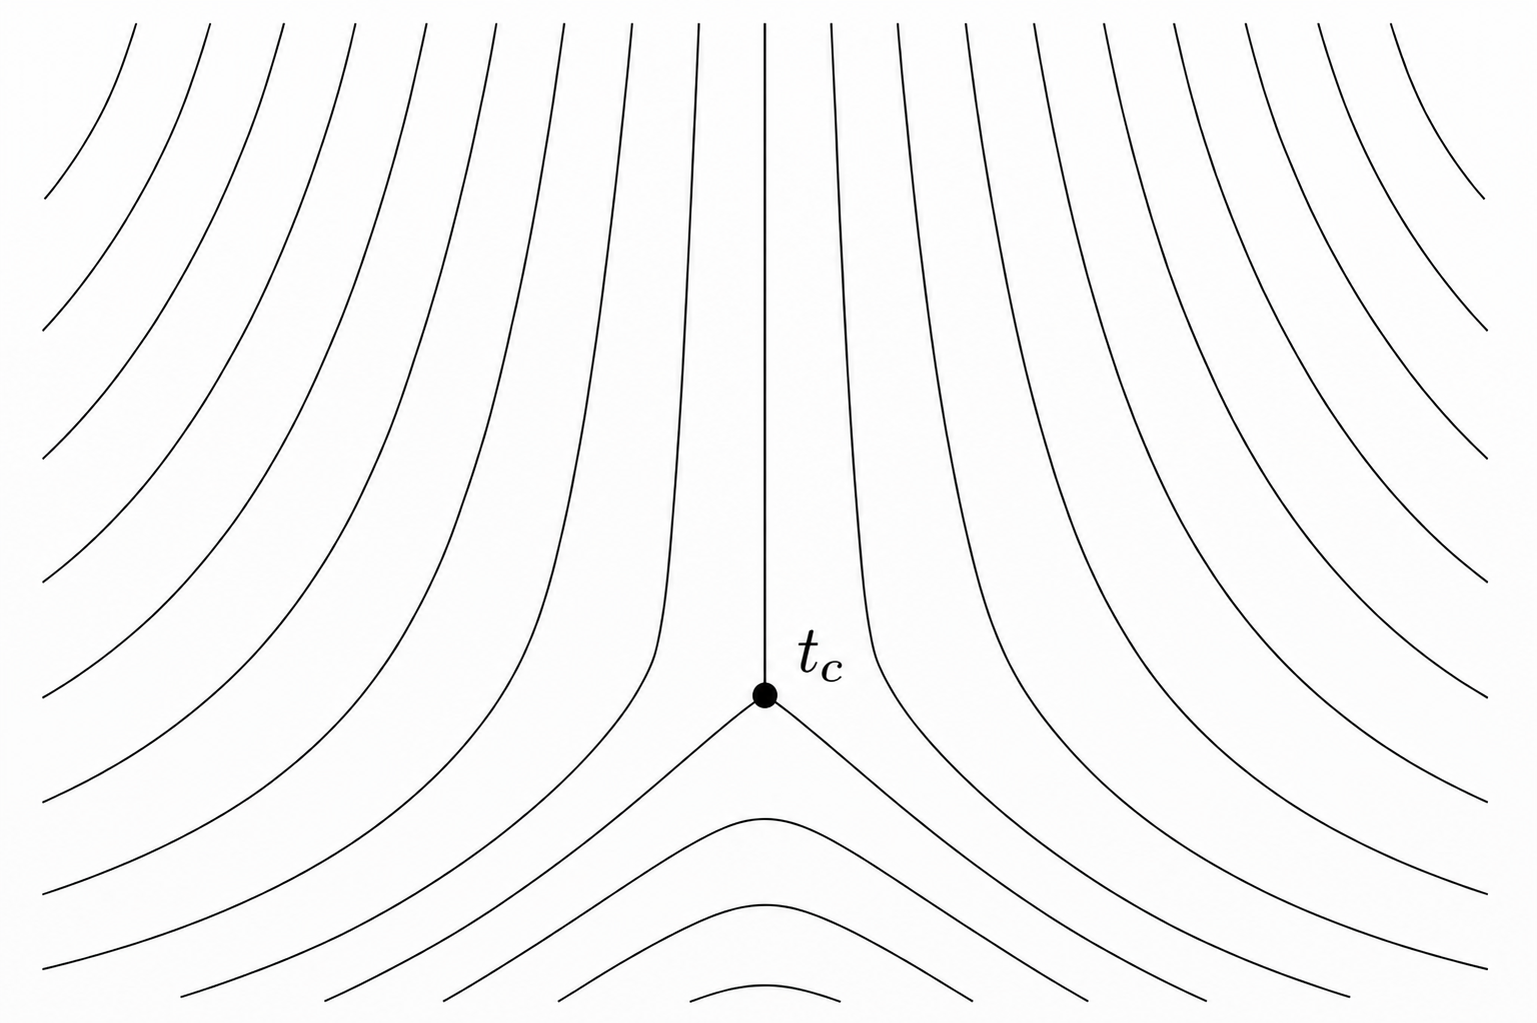
\includegraphics[width=0.5\textwidth]{level lines}
 		\caption{\textsf{Level lines of $\mathrm{Im} [\Delta (t)]$ for various constant values and the level line \newline $\mathrm{Im} [\Delta (t)] = \mathrm{Im} [\Delta (t_{c})]$ which passes through the crossing point.}}
 		\label{fig:level lines}
 	\end{figure}
 	We are now in place to specify the region $\mathcal{R}$ mentioned earlier; \emph{$\mathcal{R}$ is the region in the complex $t$-plane extending from the real axis up to the level line that passes through the closest crossing point (including the real axis and the level line as well).} \\	
	
	Having considered the eigenvalues, before moving on to considering the eigenvectors and the nonadiabatic coupling, we will write the Hamiltonian in a convenient form:
	\begin{equation}
		H = 
		\begin{pmatrix}
			H_{11} & H_{12} \\
			H_{12} & H_{22}
		\end{pmatrix}
		= \dfrac{1}{2}
		\begin{pmatrix}
			H_{11} + H_{22} & 0 \\
			0 & H_{11} + H_{22}
		\end{pmatrix}
		+ \dfrac{1}{2}
		\begin{pmatrix}
			H_{11} - H_{22} & 2H_{12} \\
			2H_{12} & H_{11} - H_{22}
		\end{pmatrix}
	\end{equation}
	which can then be written as
	\begin{equation}
		H = \bar{E} \mathbb{I} + \dfrac{1}{2} 
		\begin{pmatrix}
			H_{11} - H_{22} & 2H_{12} \\
			2H_{12} & -H_{11} + H_{22}
		\end{pmatrix}
	\end{equation}
	We now define
	\begin{equation}
		\tan(\theta) \equiv -\dfrac{2H_{12}}{H_{11} - H_{22}} \label{3.50}
	\end{equation}
	Using the exponential form, we can $\tan(\theta) = \dfrac{\sin(\theta)}{\cos(\theta)} = \dfrac{1}{i} \dfrac{e^{i\theta} - e^{-i\theta}}{e^{i\theta} + e^{-i\theta}}$ we get
	\begin{equation}
		\dfrac{e^{2i\theta} - 1}{e^{2i\theta} + 1} = -i \dfrac{2H_{12}}{H_{11} - H_{22}}
	\end{equation}
	With a little algebra, we get
	\begin{equation}
		e^{2i\theta} = \dfrac{H_{11} - H_{22} - 2iH_{12}}{H_{11} - H_{22} + 2iH_{12}} \label{3.52}
	\end{equation}
	Let us rewrite the Hamiltonian in terms of $\theta$; First, from \eqref{3.26} we can once factor $-\left( H_{11} - H_{22} \right)$ and write $\delta E$ accordingly, and once, we can factor out $2H_{12}$. We get
	\begin{equation}
		\delta E = -\left( H_{11} - H_{22} \right) \sqrt{1 + 
	\tan^{2}(\theta)} = -\left( H_{11} - H_{22} \right) \dfrac{1}{\left| \cos(\theta) \right|}
	\end{equation}
	or
	\begin{equation}
		\delta E = 2H_{12} \sqrt{1 + cot^{2}(\theta)} = 2H_{12} \dfrac{1}{\left| \sin(\theta) \right|}
	\end{equation}
	Selecting $\theta$ to be some arbitrary angle on $[0, \frac{\pi}{2})$, we can bring out the $\sin$ and $\cos$ from the absolute values and write the Hamiltonian in the following way:
	\begin{equation}
		H(t) = \bar{E} \mathbb{I} + \dfrac{\delta E}{2}
		\begin{pmatrix}
			-\cos(\theta) & \sin(\theta) \\
			\sin(\theta) & \cos(\theta)
		\end{pmatrix} \label{3.55}
	\end{equation}
	To find the eigenvectors of the Hamiltonian, we first solve for the eigenvalues of $H$. In fact, we do not even need to solve the eigenvalue equation for $H$, just the second expression, because the first terms proportional to the identity, just shifts the energy levels by a constant and does not alter the eigenvectors. Thus, we will just find the eigenvalues and eigenvectors of the second matrix in \eqref{3.55}. The eigenvalues of the matrix in \eqref{3.55} are $\pm 1$. The eigenvalues are calculated using the eigenvalue equations. For $\left| \chi_{1} \right\rangle$, we have
	\begin{equation}
		\begin{pmatrix}
			-\cos(\theta) + 1 & \sin(\theta) \\
			\sin(\theta) & \cos(\theta) + 1
		\end{pmatrix}
		\begin{pmatrix}
			a \\
			b
		\end{pmatrix}
		= 0 \quad \Rightarrow \quad a = -\dfrac{\sin(\theta)}{1 - \cos(\theta)} b = -\cot(\frac{\theta}{2}) b
	\end{equation}
	And from normalizing the eigenvectors, we have the condition $\left| a \right|^{2} + \left| b \right|^{2} = 1$ (Remember that $a$ and $b$ are both real (refer to the argument in the footnote (1) in \ref{subsec:setup})). From these, we get
	\begin{equation}
		b = \dfrac{1}{\sqrt{1 + \cot^{2}\left( \frac{\theta}{2}  \right)}} = -\sin(\frac{\theta}{2})
	\end{equation}
	The sign choice is arbitrary. From this, we find $a = \cos(\frac{\theta}{2})$ and thus
	\begin{equation}
		\left| \chi_{1} \right\rangle = \pm
		\begin{pmatrix}
			\cos(\frac{\theta}{2}) \\[5pt]
			-\sin(\frac{\theta}{2})
		\end{pmatrix}
	\end{equation}
	The arbitrary sign (which, in general, is a phase) will be chosen later. The calculations for $\left| \chi_{2} \right\rangle$ are similar and we get
	\begin{equation}
		\left| \chi_{2} \right\rangle = \pm
		\begin{pmatrix}
			\sin(\frac{\theta}{2}) \\[5pt]
			\cos(\frac{\theta}{2})
		\end{pmatrix}
	\end{equation}
	Again, there is a redundancy of sign which will be resolved shortly.
	Now that we have found the eigenvectors, we can calculate the nonadiabatic coupling \eqref{3.19}:
	\begin{equation}
		\gamma(t) = \pm 
		\begin{pmatrix}
			\cos(\frac{\theta}{2}) & -\sin(\frac{\theta}{2})
		\end{pmatrix}
		\begin{pmatrix}
			\cos(\frac{\theta}{2}) \\[5pt]
			-\sin(\frac{\theta}{2})
		\end{pmatrix}
		\left( \dfrac{\theta'}{2} \right)
	\end{equation}
	Note that $\theta$ is a function of $t$.
	\begin{equation}
		\gamma(t) = \pm \dfrac{\theta'}{2}
	\end{equation}
	How does $\gamma$ behave around the crossing point? Look back at \eqref{3.28}; So, at the crossing point, either the numerator or the denominator of the expression in \eqref{3.52} vanish. Also, remember from \eqref{3.32} that in a close neighborhood of $t_{c}$, $\delta E$ behaves as $\left( t - t_{c} \right)^{\frac{1}{2}}$ and hence
	\begin{equation}
		\left( \delta E \right)^{2} \sim t - t_{c} \label{3.62}
	\end{equation}
	Also from \eqref{3.26} we have
	\begin{equation}
		\left( \delta E \right)^{2} = \left( H_{11} - H_{22} - 2i H_{12} \right) \left( H_{11} - H_{22} + 2i H_{12} \right) \label{3.63}
	\end{equation}
	Remember that, generally, not both the parenthesis in \eqref{3.63} vanish simultaneously at $t_{c}$; either the first parentheses vanishes at $t_{c}$ and the second parentheses is analytic at $t_{c}$, or, vice versa. We will consider the both cases: First, let us assume that the numerator in \eqref{3.52} vanishes at $t_{c}$. In a close neighborhood of $t_{c}$, the left-hand side of \eqref{3.63} behaves as $t-t_{c}$ and so the numerator in \eqref{3.52} must behave as $t-t_{c}$ as well. So, using \eqref{3.52}, we have
	\begin{equation}
		e^{2i\theta} = \dfrac{t - t_{c}}{D(t)}
	\end{equation}
	Where $D(t)$ is some function that is analytic at $t_{c}$. Then taking the logarithm of both sides gives
	\begin{equation}
		2i\theta = \ln(t-t_{c}) - \ln(D(t))
	\end{equation}
	differentiating both sides with respect to $t$ and diving by $4i$ gives
	\begin{equation}
		\frac{\theta'}{2} = \dfrac{1}{4i \left( t - t_{c} \right)} - \dfrac{D'(t)}{4iD(t)} \label{3.66}
	\end{equation}
	What if the denominator vanishes at $t_{c}$? In that case, we would have
	\begin{equation}
		e^{2i\theta} = \dfrac{N(t)}{t - t_{c}}
	\end{equation}
	Where $N(t)$ is some other function that is analytic at $t_{c}$. Carrying on similarly as we did above, we get
	\begin{equation}
			\frac{\theta'}{2} = -\dfrac{1}{4i \left( t - t_{c} \right)} + \dfrac{N'(t)}{4iN(t)} \label{3.68}
	\end{equation}
	So in a close vicinity of $t_{c}$, we have
	\begin{equation}
		\frac{\theta'}{2} = \pm \dfrac{1}{4i \left( t-t_{c} \right)}
	\end{equation}
	We will select the relative sign of the eigenvectors such that it results in the $+$ sign in the above expression. Therefore, the behavior the nonadiabatic coupling in a neighborhood of $t_{c}$ is determined by
	\begin{equation}
		\boxed{\gamma(t) = \dfrac{1}{4i \left( t-t_{c} \right)} + \eta(t)} \label{3.70}
	\end{equation}
	Where $\eta(t)$ is some function that is analytic at $t_{c}$\footnote{Where does $\eta(t)$ come from? In \eqref{3.66} and \eqref{3.68}, there were expressions that involved $N(t)$ or $D(t)$; Those expressions are analytic at $t_{c}$ and thus, in the final expression in \eqref{3.70}, We introduce $\eta(t)$ to capture the behavior of $\gamma$ beyond the leading term that is proportional to $\frac{1}{t-t_{c}}$.}. Notice that the leading term in the nonadiabatic coupling is a simple pole at $t_{c}$ with residue that is independent of the form of the Hamiltonian. This feature will ultimately result in a transition amplitude that is independent of $\gamma$. This doesn't mean that the nonadiabatic coupling is unimportant, but that, in its leading term, is the same for all problems. Further, we will assume that \emph{$\gamma$, $\left( \frac{\gamma}{\delta E} \right)'$ and $\frac{\gamma^{2}}{\delta E}$ are absolutely integrable along the real axis and along the level lines of $\mathrm{Im} \Delta (t)$ that pass through the crossing point $t_{c}$.} \\
	
	In the next section, we will first begin by integrating equations \eqref{3.22} and \eqref{3.33} on the real-time domain and then move to the complex plane for a more informative analysis. 
	
	\section{Calculation of the coefficients in the semiclassical limit}
	\label{sec:calculation}
	
	\subsection{Finite-time analysis on the real axis} \label{subsec:real analysis}
	
	We want to solve for the coefficients at time $t$ from equations \eqref{3.22} and \eqref{3.23}. The initial conditions are $a_{1}(-\infty) = 1$ and $a_{2}(-\infty) = 0$ and that $\gamma(-\infty) = 0$. Integrating from $-\infty$ to some finite $t$	
	\begin{align}
		\int_{-\infty}^{t} d\tau \, a_{2}'(\tau) &= \int_{-\infty}^{t} d\tau \, \gamma(\tau) \exp\left( \frac{i}{\hbar} \Delta(\tau) \right) \, a_{1}(\tau) \\[5pt]
		\int_{-\infty}^{t} d\tau \, a_{1}'(\tau) &= -\int_{-\infty}^{t} d\tau \, \gamma(\tau) \exp\left( -\frac{i}{\hbar} \Delta(\tau) \right) \, a_{2}(\tau)
	\end{align}
	which yields
	\begin{align}
		a_{2}(t) &= \int_{-\infty}^{t} d\tau \, \gamma(\tau) \exp\left( \frac{i}{\hbar} \Delta(\tau) \right) \, a_{1}(\tau) \label{4.3} \\[5pt]
		a_{1}(t) - 1 &= -\int_{-\infty}^{t} d\tau \, \gamma(\tau) \exp\left( -\frac{i}{\hbar} \Delta(\tau) \right) \, a_{2}(\tau) \label{4.4}
	\end{align}
	We are going to use integration by parts here. With some hindsight, we propose an ansatz and then differentiate it:
	\begin{align}
		\left( \dfrac{\hbar}{i \delta E(t)} \gamma(t) \exp\left( \dfrac{i}{\hbar} \Delta(t) \right) a_{1}(t) \right)' &= \dfrac{\hbar}{i} \left( \dfrac{\gamma}{\delta E} \right)' \exp\left( \dfrac{i}{\hbar} \Delta \right) a_{1} \notag \\ 
		&+ \gamma \exp\left( \dfrac{i}{\hbar} \Delta \right) a_{1} \notag \\
		&+ \dfrac{\hbar}{i \delta E} \gamma \exp\left( \dfrac{i}{\hbar} \Delta \right) a_{1}' \label{4.5}
	\end{align}
	Where we have differentiated term-by-term and used, from \eqref{3.33}, that $\Delta'(t) = \delta E(t)$. The second term on the right-hand side is exactly the integrand in \eqref{4.3} and now we can perform the integration by parts by substituting for the integrand, using \eqref{4.5}:
	\begin{align}
		a_{2}(t) &= \int_{-\infty}^{t} d\tau \, \gamma \exp\left( \frac{i}{\hbar} \Delta \right) \, a_{1} \notag \\[5pt]
		&= \int_{-\infty}^{t} d\tau \,\left( \dfrac{\hbar}{i \delta E} \gamma \exp\left( \dfrac{i}{\hbar} \Delta \right) a_{1} \right)' \notag \\[5pt]
		&- \int_{-\infty}^{t} d\tau \, \dfrac{\hbar}{i} \left( \dfrac{\gamma}{\delta E} \right)' \exp\left( \dfrac{i}{\hbar} \Delta \right) a_{1} \notag \\[5pt]
		&- \int_{-\infty}^{t} d\tau \, \dfrac{\hbar}{i \delta E} \gamma \exp\left( \dfrac{i}{\hbar} \Delta \right) a_{1}'
	\end{align}
	Upon evaluating the first term on the right-hand side and substituting for $a_{1}'$ from \eqref{3.23}, we get
	\begin{align}
		a_{2}(t) &= \dfrac{\hbar}{i} \dfrac{\gamma(t)}{\delta E(t)} \exp\left( \dfrac{i}{\hbar} \Delta(t) \right) a_{1}(t) \notag \\[5pt]
		&- \dfrac{\hbar}{i} \int_{-\infty}^{t} d\tau \, \left( \dfrac{\gamma}{\delta E} \right)' \exp\left( \dfrac{i}{\hbar} \Delta \right) a_{1} \notag \\[5pt]
		&+ \dfrac{\hbar}{i} \int_{-\infty}^{t} d\tau \, \dfrac{\gamma^{2}}{\delta E} \,  a_{2}  \label{4.7}
	\end{align}
	Since $\gamma(-\infty) = 0$. We expect, from the adiabatic theorem, that $a_{2} \xrightarrow[\hbar \rightarrow 0]{} 0$ but the question is \textquotedblleft how rapidly?\textquotedblright. First off, $\exp\left( \frac{i}{\hbar} \Delta \right)$ has magnitude equal to $1$ (Since $\Delta$ is real on the real time axis). Second, The magnitude of the coefficients is always less than or equal to $1$ (A direct consequence of the fact that the state of the system is normalizable). Thus, using the triangular inequality, we can get
	\begin{align}
		\left| a_{2}(t) \right| &\leq \hbar \left| \dfrac{\gamma(t)}{\delta E(t)} \exp\left( \dfrac{i}{\hbar} \Delta(t) \right) a_{1}(t) \right| \notag \\[5pt]
		&+ \hbar \left| \int_{-\infty}^{t} d\tau \, \left( \dfrac{\gamma}{\delta E} \right)' \exp\left( \dfrac{i}{\hbar} \Delta \right) a_{1} \right| \notag \\[5pt]
		&+ \hbar \left| \int_{-\infty}^{t} d\tau \, \dfrac{\gamma^{2}}{\delta E} \,  a_{2} \right| \notag \\[5pt]
		&\leq \hbar \left[ \left| \dfrac{\gamma(t)}{\delta E(t)} \right| + \int_{-\infty}^{t} d\tau \, \left| \left( \dfrac{\gamma}{\delta E} \right)' \right| + \int_{-\infty}^{t} d\tau \,  \left| \dfrac{\gamma^{2}}{\delta E} \right| \right] \label{4.8}
	\end{align}
	Defining
	\begin{equation}
		C \equiv \mathrm{max}_{t} \left| \dfrac{\gamma(t)}{\delta E(t)} \right| + \int_{-\infty}^{\infty} d\tau \, \left| \left( \dfrac{\gamma}{\delta E} \right)' \right| + \int_{-\infty}^{\infty} d\tau \, \left| \dfrac{\gamma^{2}}{\delta E} \right| \label{4.9}
	\end{equation}
	($\mathrm{max}_{t}$ returns the maximum value of the argument (for all $t$) passed to it.). With the remarks made at the end of \ref{subsec:behavior of functions}, we can deduce that the right-hand side of \eqref{4.9} is some finite number and thus
	\begin{equation}
		\left| a_{2}(t) \right| \leq \hbar C \label{4.10}
	\end{equation}
	Working on \eqref{4.4} gives
	\begin{align}
		\left| a_{1}(t) - 1 \right| &\leq \left| \int_{-\infty}^{t} d\tau \, \gamma(\tau) \exp\left( \frac{i}{\hbar} \Delta(\tau) \right) \, a_{2}(\tau) \right| \notag \\[5pt]
		&\leq \hbar C \int_{-\infty}^{\infty} d\tau \, \left| \gamma(\tau) \right| = \hbar C' \label{4.11}
	\end{align}
	Where
	\begin{equation}
		C' \equiv C \int_{-\infty}^{\infty} d\tau \, \left| \gamma(\tau) \right|
	\end{equation}
	(Assuming $\gamma(t)$ is a well-behaved and absolutely integrable function on the real rime axis.). We will now work on the integrals on the right-hand side of \eqref{4.7}.
	\begin{equation}
		\int_{-\infty}^{t} d\tau \, \left( \dfrac{\gamma}{\delta E} \right)' \exp\left( \dfrac{i}{\hbar} \Delta \right) a_{1} = \int_{-\infty}^{t} d\tau \, \left( \dfrac{\gamma}{\delta E} \right)' \exp\left( \dfrac{i}{\hbar} \Delta \right) \left( a_{1} - 1 \right) + \int_{-\infty}^{t} d\tau \, \left( \dfrac{\gamma}{\delta E} \right)' \exp\left( \dfrac{i}{\hbar} \Delta \right) \label{4.13}
	\end{equation}
	The second integral on the right-hand side goes to $0$ as $\hbar$ approaches $0$ by the Riemann-Lebesgue lemma \footnote{The statement of the lemma in one dimension is as follows: Suppose an absolutely integrable function $f(x)$ on the real axis $x$; that is
	\begin{equation}
		\int_{-\infty}^{\infty} dx\, \left| f(x) \right| < \infty \notag
	\end{equation}
	And now consider the Fourier transform of this function
	\begin{equation}
		\widetilde{f}(\xi) = \int_{-\infty}^{\infty} dx\, f(x)\, e^{-i\xi x} \notag
	\end{equation}
	The lemma states that $\left| \widetilde{f}(\xi) \right| \rightarrow 0$ as $\left| \xi \right| \rightarrow \infty$.
	Expressions in the main text have $\hbar^{-1} \sim \xi$.
	}. For the first one, we have
	\begin{align}
		\left| \int_{-\infty}^{t} d\tau \, \left( \dfrac{\gamma}{\delta E} \right)' \exp\left( \dfrac{i}{\hbar} \Delta \right) \left( a_{1} - 1 \right) \right| &\leq \left| a_{1} - 1 \right| \left| \int_{-\infty}^{t} d\tau \, \left( \dfrac{\gamma}{\delta E} \right)' \exp\left( \dfrac{i}{\hbar} \Delta \right) \right| \notag \\[5pt]
		&\leq \hbar C' \left| \int_{-\infty}^{t} d\tau \, \left( \dfrac{\gamma}{\delta E} \right)' \exp\left( \dfrac{i}{\hbar} \Delta \right) \right| \xrightarrow[\hbar \rightarrow 0]{} 0
	\end{align}
	Since the integral is finite. Now for the second integral in \eqref{4.7}, we have
	\begin{equation}
		\left| \int_{-\infty}^{t} d\tau \, \dfrac{\gamma^{2}}{\delta E} \,  a_{2} \right| \leq \hbar C \left| \int_{-\infty}^{t} d\tau \, \dfrac{\gamma^{2}}{\delta E} \right| \xrightarrow[\hbar \rightarrow 0]{} 0
	\end{equation}
	Again, since the integral is finite. Thus, we can deduce that (looking back at \eqref{4.7} and noting that $a_{1} \sim 1$ as $\hbar \rightarrow 0$)
	\begin{equation}
		\boxed{a_{2}(t) \sim \hbar \dfrac{\gamma(t)}{i \delta E(t)} \exp\left( \dfrac{i}{\hbar} \Delta(t) \right)} \label{4.16}
	\end{equation}
	All fair and well. This form of convergence gives insight about the behavior of $a_{2}$ and consecutively, the transition amplitude and validates that $a_{2}(t) \rightarrow 0$ as $\hbar \rightarrow 0$ but carries less information when considered in the limit where $t \rightarrow \infty$ (where $\gamma = 0$). In the next subsection, we will take up that problem and move to the complex plane for a more involved and informative analysis. \\
	
	Remark: \emph{For the upcoming calculations, we will denote finite constants that are independent of $\hbar$ with $C_{1}, C_{2}, \cdots$.}  
	
	\subsection{Using contour integration and the complex-time approach} \label{subsec:complex analysis}
	
	Our starting point is the system of differential equation \eqref{3.22} and \eqref{3.23} ($t$ is a complex variable). For more convenience, we define
	\begin{equation}
		\tilde{a}_{1}(t, \hbar) \equiv a_{1}(t, \hbar) \qquad , \qquad \tilde{a}_{2}(t, \hbar) \equiv \exp\left(- \dfrac{i}{\hbar} \Delta_{c} \right) a_{2}(t, \hbar) \label{4.17}
	\end{equation}
	Where $\Delta_{c} = \Delta (t_{c})$. Rewriting the equation in terms of the new coefficients will give us
	\begin{align}
		\tilde{a}_{2}'(t) &= \gamma(t) \exp\left( \dfrac{i}{\hbar} \left[ \Delta(t) - \Delta_{c} \right] \right) \tilde{a}_{1}(t) \label{4.18} \\
		\tilde{a}_{1}'(t) &= -\gamma(t) \exp\left(- \dfrac{i}{\hbar} \left[ \Delta(t) - \Delta_{c} \right] \right) \tilde{a}_{2}(t) \label{4.19}
	\end{align}
	The initial conditions are $\tilde{a}_{1}(-\infty) = 1$ and $\tilde{a}_{2}(-\infty) = 0$. Also, we will adopt a short-hand notation for the exponentials appearing in \eqref{4.18} and \eqref{4.19}:
	\begin{equation}
		\exp\left( \pm \dfrac{i}{\hbar} \left[ \Delta(t) - \Delta_{c} \right] \right) \equiv e^{\pm} \label{4.20}
	\end{equation}
	The goal is to find $a_{2}(\infty)$ and from that, the transition amplitude $\mathcal{P}_{1 \rightarrow 2} = \left| a_{2}(\infty) \right|^{2}$. For that purpose, we need to evaluate integrals on (real) $t$ from $-\infty$ to $\infty$ but since the integrands are analytic throughout the region $\mathcal{R}$ in the complex plane, the integrals (integrating \eqref{4.18} and \eqref{4.19}) are path-independent and thus, we choose to evaluate the integrals along the contour specified below:
	\begin{figure}[H]
		\centering
		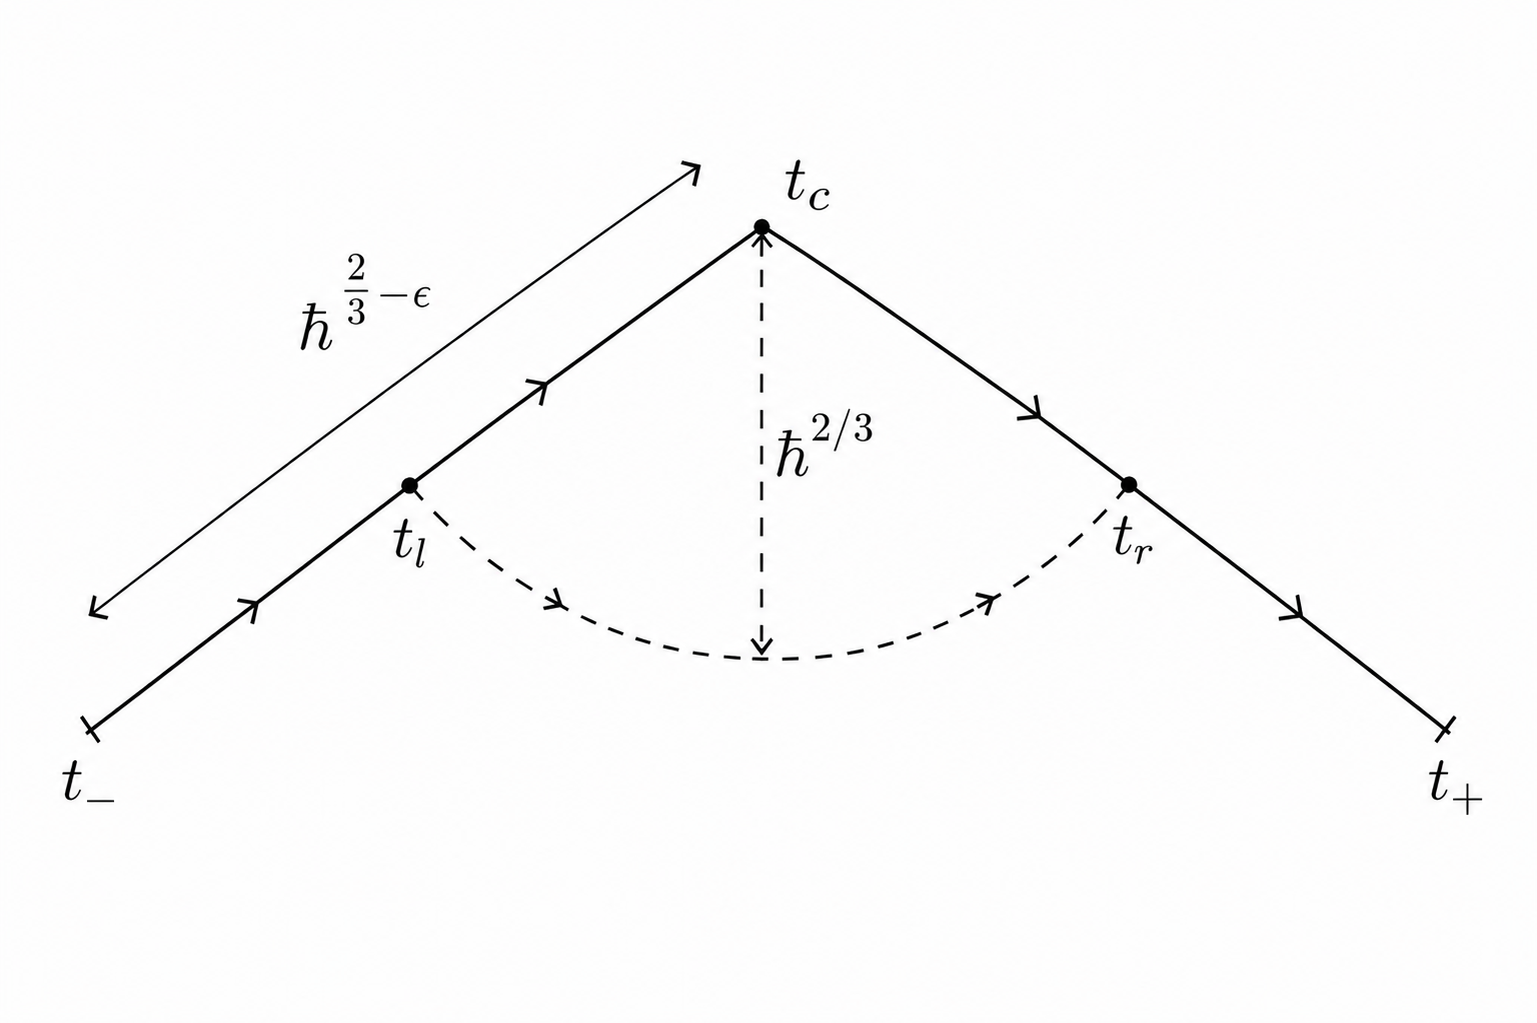
\includegraphics[width = 0.65\textwidth]{contour}
		\caption{\textsf{The integration contour $\mathcal{C}$; \emph{The left tail} from $-\infty$ to $t_{-}$ where $\left| t_{-} - t_{c} \right| = \hbar^{\frac{2}{3} - \epsilon}$ , the center contour which itself is composed of \emph{the left arm} from $t_{-}$ to $t_{l}$, \emph{the dip} from $t_{l}$ to $t_{r}$ (on the arc of the circle with radius $\hbar^{\frac{2}{3}}$ and center at $t_{c}$) and \emph{the right arm} from $t_{r}$ to $t_{+}$ (where $\left| t_{+} - t_{c} \right| = \hbar^{\frac{2}{3} - \epsilon}$), and \emph{the right tail} from $t_{+}$ to $\infty$. All segments of $\mathcal{C}$ are along the level line of $\mathrm{Im}[\Delta(t)]$ (more specifically, the level line where $\mathrm{Im}[\Delta(t)] = \mathrm{Im}[\Delta_{c}]$) except for the detour below $t_{c}$ (the dashed curve). $\epsilon$ is a small, positive constant (which will be specified later in the calculations).}}
	\end{figure}
	From \eqref{4.18} and \eqref{4.19}, we get
	\begin{align}
		\tilde{a}_{2}(t) = \int^{t} d\tau \, \gamma\, e^{+}\, \tilde{a}_{1} &= \dfrac{\hbar}{i} \dfrac{\gamma(t)}{\delta E(t)}\, e^{+}\, \tilde{a}_{1}(t) \notag \\[5pt]
		&- \dfrac{\hbar}{i} \int^{t} d\tau \, \left( \dfrac{\gamma}{\delta E} \right)'\, e^{+}\, \tilde{a}_{1} \notag \\[5pt]
		&+ \dfrac{\hbar}{i} \int^{t} d\tau \, \dfrac{\gamma^{2}}{\delta E} \,  \tilde{a}_{2} \label{4.21}
	\end{align}
	And
	\begin{align}
		\tilde{a}_{1}(t) - 1 = -\int^{t} d\tau \, \gamma\, e^{-}\, \tilde{a}_{2} &= \dfrac{\hbar}{i} \dfrac{\gamma(t)}{\delta E(t)}\, e^{-}\, \tilde{a}_{2}(t) \notag \\[5pt]
		&- \dfrac{\hbar}{i} \int^{t} d\tau \, \left( \dfrac{\gamma}{\delta E} \right)'\, e^{-}\, \tilde{a}_{2} \notag \\[5pt]
		&- \dfrac{\hbar}{i} \int^{t} d\tau \, \dfrac{\gamma^{2}}{\delta E} \,  \tilde{a}_{1} \label{4.22}
	\end{align}
	$t$ is any point on the left tail to the left of $t_{-}$.
	
	We want to show that, in the semiclassical/adiabatic limit, the integration on the center contour contributes more significantly to the integrals than the tails; In other words, we would like to show that the coefficients $\tilde{a}_{1}$ and $\tilde{a}_{2}$ are asymptotically constant along the left and the right tails. To verify this fact, it suffices to show that the coefficients remain (asymptotically) constant along the left tail of the contour $\mathcal{C}$, because, then, by symmetry arguments, we can come at a similar conclusion for the right tail of $\mathcal{C}$.
	
	Let us introduce some quantities:
	\begin{equation}
		\mathcal{M}_{1} \equiv \mathrm{max}_{\leq t_{-}} \left| \tilde{a}_{1} - 1 \right| \qquad , \qquad \mathcal{M}_{2} \equiv \mathrm{max}_{\leq t_{-}} \left| \tilde{a}_{2} \right| \label{4.23}
	\end{equation}
	And
	\begin{equation}
		\mathcal{A}_{1} \equiv \mathrm{max}_{\leq t_{-}} \left| \dfrac{\gamma}{\delta E} \right| \, , \, \mathcal{A}_{2} \equiv \int^{t_{-}} \left| d\tau \right| \left| \left( \dfrac{\gamma}{\delta E} \right)' \right| \, , \, \mathcal{A}_{3} \equiv \int^{t_{-}} \left| d\tau \right| \left| \dfrac{\gamma^{2}}{\delta E} \right| \label{4.24}
	\end{equation}
	$\mathrm{max}_{\leq t_{-}}$ returns to the maximum of the argument for all $t$ along the left tail to the left of $t_{-}$. We can readily obtain the inequality $\left| \tilde{a}_{1} \right| \leq 1 + \mathcal{M}_{1}$. From \eqref{4.21} and \eqref{4.22}, we can get \footnote{Using the handy triangular inequality and
	\begin{equation}
		\left| \int_{\mathcal{C}} f(t)\, dt \right| \leq \int_{\mathcal{C}} \left| f(t) \right|\, \left| dt \right| \notag
	\end{equation}
	Which itself, in essence, is obtained from the triangular inequality (By writing the integral as a sum and then employing the generalized triangular inequality).} \footnote{Note that the exponentials all have magnitude equal to $1$. Why is that? Looking back at \eqref{4.20} and remembering that the left tail is part of the level line where $\mathrm{Im}[\Delta(t)] = \mathrm{Im}[\Delta_{c}]$, $e^{\pm}$ are simply $\exp\left( \pm \frac{i}{\hbar} \mathrm{Re}\left[ \Delta(t) - \Delta_{c} \right] \right)$ which always has magnitude equal to $1$. \label{footnote:8}} 
	\begin{align}
		\left| \tilde{a}_{2} \right| &\leq \hbar \left[ \left| \dfrac{\gamma}{\delta E} \right| \left| \tilde{a}_{1} \right| + \int^{t} \left| d\tau \right| \left| \left( \dfrac{\gamma}{\delta E} \right)' \right| \left| \tilde{a}_{1} \right| + \int^{t} \left| d\tau \right| \left| \dfrac{\gamma^{2}}{\delta E} \right| \left| \tilde{a}_{2} \right| \right] \label{4.25} \\[5pt]
		\left| \tilde{a}_{1} - 1 \right| &\leq \hbar \left[ \left| \dfrac{\gamma}{\delta E} \right| \left| \tilde{a}_{2} \right| + \int^{t} \left| d\tau \right| \left| \left( \dfrac{\gamma}{\delta E} \right)' \right| \left| \tilde{a}_{2} \right| + \int^{t} \left| d\tau \right| \left| \dfrac{\gamma^{2}}{\delta E} \right| \left| \tilde{a}_{1} \right| \right] \label{4.26}
	\end{align}
	And further, since the values of the coefficients (for all $t$) on the left tail satisfies the inequalities \eqref{4.25} and \eqref{4.26}, their maximum values will also satisfy the inequalities:
	\begin{align}
		\mathcal{M}_{2} &\leq \hbar \left[ \left( \mathcal{A}_{1} + \mathcal{A}_{2} \right) \left( 1 + \mathcal{M}_{1} \right) + \mathcal{A}_{3}\mathcal{M}_{2} \right] \label{4.27} \\[5pt]
		\mathcal{M}_{1} &\leq \hbar \left[ \left( \mathcal{A}_{1} + \mathcal{A}_{2} \right) \mathcal{M}_{2} + \mathcal{A}_{3}\left( 1 + \mathcal{M}_{1} \right) \right] \label{4.28}
	\end{align}
	We will now find upper-bounds for the $\mathcal{A}$'s, starting with $\mathcal{A}_{1}$. We will have in mind, the expressions \eqref{3.32} and \eqref{3.70}. We want to maximize the expression $\left| \frac{\gamma}{\delta E} \right|$, we may obtain this by attempting to maximize the numerator and minimize the denominator. For the denominator, we have a series expansion given by \eqref{3.32}; to minimize $\delta E$, we will focus only on the first term that is proportional to $\left( t - t_{c} \right)^{\frac{1}{2}}$. For the numerator, we will consider the leading term in \eqref{3.70}\footnote{Why? what if the contribution from $\eta$ becomes more noticeable than that of the leading term? Well, that is a fair concern but note that $\eta$ is analytic at $t_{c}$ and throughout the region $\mathcal{R}$, so we can always find an upper-bound $C_{1}$ such that $\left| \eta(t) \right| \leq C_{1}$ for all t along the left tail but as we get closer and closer to the crossing point, the magnitude of the expression $\left( t - t_{c} \right)^{-1}$ increases without bound and becomes larger than any finite constant (As $\hbar \rightarrow 0$) and hence, the contribution from the leading term dominates. Similar arguments will hold for $\mathcal{A}_{2}$ and $\mathcal{A}_{3}$. In general, the behavior around $t_{c}$ is of special interest since the more prominent effects, take place there.}. Thus (in a close vicinity of $t_{c}$)
	\begin{equation}
		\left| \dfrac{\gamma}{\delta E} \right| \sim \left| \dfrac{\left( t - t_{c} \right)^{-1}}{\left( t - t_{c} \right)^{\frac{1}{2}}} \right| \sim \left| \left( t - t_{c} \right)^{-\frac{3}{2}}\right| \leq C_{2} \left| t_{-} - t_{c} \right|^{-\frac{3}{2}} = C_{2} \left( \hbar^{\frac{2}{3} - \epsilon} \right)^{-\frac{3}{2}} = C_{2}\, \hbar^{\frac{3}{2}\epsilon - 1} \label{4.29}
	\end{equation}
	And therefore, we can write
	\begin{equation}
		\mathcal{A}_{1} \leq C_{2}\, \hbar^{\frac{3}{2}\epsilon - 1} \label{4.30}
	\end{equation}
	Now $\mathcal{A}_{2}$. In a close neighborhood of $t_{c}$
	\begin{equation}
		\dfrac{\gamma}{\delta E} \sim \left( t - t_{c} \right)^{-\frac{3}{2}} \label{4.31}
	\end{equation}
	Differentiating the above expression with respect to $t$ gives
	\begin{equation}
		\left( \dfrac{\gamma}{\delta E} \right)' \sim \left( t - t_{c} \right)^{-\frac{5}{2}} \quad \rightarrow \quad \left| \left( \dfrac{\gamma}{\delta E} \right)' \right| \sim \left| t - t_{c} \right|^{-\frac{5}{2}} \label{4.32}
	\end{equation}
	And now we can estimate how the integral behaves \footnote{The integral from $-\infty$ to some fixed point (to the left of $t_{-}$ gives a finite number independent of $\hbar$ (Since the function is assumed to be absolutely integrable along the left tail) and from that fixed point to $t_{-}$, we have the expression for it given in \eqref{4.33}).}:
	\begin{equation}
		\int^{t_{-}} \left| d\tau \right| \left| \left( \dfrac{\gamma}{\delta E} \right)' \right| \sim \int^{t_{-}} \left| d\tau \right| \left| \tau - t_{c} \right|^{-\frac{5}{2}} \label{4.33}
	\end{equation}
	which is easily integrable (A straightforward change of variable to $\tau - t_{c}$ gives a trivial integral) and 
	\begin{equation}
		\int^{t_{-}} \left| d\tau \right| \left| \left( \dfrac{\gamma}{\delta E} \right)' \right| \sim \left| t - t_{c} \right|^{-\frac{3}{2}} \label{4.34}
	\end{equation}
	And now we can write
	\begin{equation}
		\mathcal{A}_{2} \leq C_{3}\, \left| t_{-} - t_{c} \right|^{-\frac{3}{2}} = C_{3}\, \left( \hbar^{\frac{2}{3} - \epsilon} \right)^{-\frac{3}{2}} = C_{3}\, \hbar^{\frac{3}{2}\epsilon - 1} \label{4.35}
	\end{equation}
	And finally, $\mathcal{A}_{3}$. In a close neighborhood of $t_{c}$, we have
	\begin{equation}
		\dfrac{\gamma^{2}}{\delta E} \sim \left( t - t_{c} \right)^{-\frac{5}{2}}
	\end{equation}
	Pretty much like the analysis for $\mathcal{A}_{2}$ (Similar behavior of the integrand and the fact that the integrand has, a priori, been assumed to be absolutely integrable). We get
	\begin{equation}
		\mathcal{A}_{3} \leq C_{4}\, \hbar^{\frac{3}{2}\epsilon - 1}
	\end{equation}
	So all $\mathcal{A}$'s behave similarly (they are all bounded by some constant times $\hbar^{\frac{3}{2}\epsilon - 1}$) and thus, referring to \eqref{4.27} and \eqref{4.28}, we can write
	\begin{align}
		\mathcal{M}_{2} &\leq \hbar \times C_{5}\, \hbar^{\frac{3}{2}\epsilon - 1} = C_{5}\, \hbar^{\frac{3}{2}\epsilon} \label{4.38} \\
		\mathcal{M}_{1} &\leq \hbar \times C_{6}\, \hbar^{\frac{3}{2}\epsilon - 1} = C_{6}\, \hbar^{\frac{3}{2}\epsilon} \label{4.39}
	\end{align}
	The right-hand side of both these equations vanish as $\hbar \rightarrow 0$ and hence, $\mathcal{M}_{2}$ and $\mathcal{M}_{1}$ vanish in that limit as well and consequently, the coefficients are asymptotically constant up to $t_{-}$ and from $t_{+}$ to $\infty$. So the transition is localized in the vicinity of $t_{c}$ on the center contour.
	
	Back to \eqref{4.18} and \eqref{4.19} and now we will integrate along the center contour (knowing that before and after that, the coefficients remain asymptotically constant) and get
	\begin{align}
		\tilde{a}_{2}(t) &= \tilde{a}_{2}(t_{-}) + \int_{t_{-}}^{t} d\tau\, \gamma\, e^{+}\, \tilde{a}_{1} \label{4.40} \\[5pt]
		\tilde{a}_{1}(t) &= \tilde{a}_{1}(t_{-}) - \int_{t_{-}}^{t} d\tau\, \gamma\, e^{-}\, \tilde{a}_{2} \label{4.41}
	\end{align}
	$t$ is any point along the center contour. How do we solve these equations? Well, one way is to solve for the coefficients and then iteratively, substitute these solutions back in and solve again to get the higher order solution (A standard procedure in solving integral equations). The \emph{zeroth order} solutions are just the values of the coefficients at $t_{-}$; that is
	\begin{equation}
		\tilde{a}_{2}^{0}(t) = \tilde{a}_{2}(t_{-}) \qquad , \qquad \tilde{a}_{1}^{0}(t) = \tilde{a}_{1}(t_{-}) \label{4.42}
	\end{equation}
	We will substitute these solutions back into \eqref{4.40} and \eqref{4.41} (under the integral) to get the \emph{first order} solutions:
	\begin{align}
		\tilde{a}_{2}^{1}(t) &= \tilde{a}_{2}(t_{-}) + \tilde{a}_{1}(t_{-}) \int_{t_{-}}^{t} dt_{1}\, \gamma\, e^{+} \label{4.43} \\[5pt]
		\tilde{a}_{1}^{1}(t) &= \tilde{a}_{1}(t_{-}) - \tilde{a}_{2}(t_{-}) \int_{t_{-}}^{t} dt_{1}\, \gamma\, e^{-} \label{4.44}
	\end{align}
	(The zeroth order solutions can be taken outside of the integral since they are constants.) Now we plug these back into \eqref{4.40} and \eqref{4.41} to get the \emph{second order} solutions:
	\begin{align}
		\tilde{a}_{2}^{2}(t) &= \tilde{a}_{2}(t_{-}) + \int_{t_{-}}^{t} \gamma\, e^{+}\, \left( \tilde{a}_{1}(t_{-}) - \tilde{a}_{2}(t_{-}) \int_{t_{-}}^{t} dt_{2}\, \gamma\, e^{-} \right) \notag \\[5pt]
		&= \tilde{a}_{1}(t_{-}) + \tilde{a}_{1}(t_{-}) \int_{t_{-}}^{t} dt_{1}\, \gamma\, e^{+} - \tilde{a}_{2}(t_{-}) \int_{t_{-}}^{t} dt_{1}\, \gamma\, e^{+} \int_{t_{-}}^{t_{1}} dt_{2}\, \gamma\, e^{-} \label{4.45} \\[5pt]
		\tilde{a}_{1}^{2}(t) &= \tilde{a}_{1}(t_{-}) - \int_{t_{-}}^{t} \gamma\, e^{-}\, \left( \tilde{a}_{2}(t_{-}) - \tilde{a}_{1}(t_{-}) \int_{t_{-}}^{t} dt_{2}\, \gamma\, e^{+} \right) \notag \\[5pt]
		&= \tilde{a}_{1}(t_{-}) - \tilde{a}_{2}(t_{-}) \int_{t_{-}}^{t} dt_{1}\, \gamma\, e^{-} -  \tilde{a}_{1}(t_{-}) \int_{t_{-}}^{t} dt_{1}\, \gamma\, e^{-} \int_{t_{-}}^{t_{1}} dt_{2}\, \gamma\, e^{+} \label{4.46}
	\end{align}
	Iterating infinitely many times will result in
	\begin{equation}
		\begin{pmatrix}
			\tilde{a}_{1}(t_{+}) \\[5pt]
			\tilde{a}_{2}(t_{+})
		\end{pmatrix}
		=
		\begin{pmatrix}
			1_{-} && \Gamma_{-} \\[5pt]
			\Gamma_{+} && 1_{+}	 
		\end{pmatrix}
		\begin{pmatrix}
			\tilde{a}_{1}(t_{-}) \\[5pt]
			\tilde{a}_{2}(t_{-})
		\end{pmatrix} \label{4.47}
	\end{equation}
	We call the matrix in \eqref{4.47} the \emph{transition matrix} (from $t_{-}$ to $t_{+}$). The elements of this matrix are 
	\begin{align}
		1_{\pm} &= 1 - \left( \int_{t_{-}}^{t_{+}} dt_{1}\, \gamma\, e^{\pm} \int_{t_{-}}^{t_{1}} dt_{2}\, \gamma\, e^{\mp} \right) \notag \\[5pt]
		&+ \left( \int_{t_{-}}^{t_{+}} dt_{1}\, \gamma\, e^{\pm} \int_{t_{-}}^{t_{1}} dt_{2}\, \gamma\, e^{\mp} \int_{t_{-}}^{t_{2}} dt_{3}\, \gamma\, e^{\pm} \int_{t_{-}}^{t_{3}} dt_{4}\, \gamma\, e^{\mp} \right) - \cdots \label{4.48} \\[20pt]
		\Gamma_{\pm} &= \pm \left( \int_{t_{-}}^{t_{+}} dt_{1}\, \gamma\, e^{\pm} \right) \mp \left( \int_{t_{-}}^{t_{+}} dt_{1}\, \gamma\, e^{\pm} \int_{t_{-}}^{t_{1}} dt_{2}\, \gamma\, e^{\mp} \int_{t_{-}}^{t_{2}} dt_{3}\, \gamma\, e^{\pm} \right) \notag \\[5pt]
		&\pm \left( \int_{t_{-}}^{t_{+}} dt_{1}\, \gamma\, e^{\pm} \int_{t_{-}}^{t_{1}} dt_{2}\, \gamma\, e^{\mp} \int_{t_{-}}^{t_{2}} dt_{3}\, \gamma\, e^{\pm} \int_{t_{-}}^{t_{3}} dt_{4}\, \gamma\, e^{\mp} \int_{t_{-}}^{t_{4}} dt_{5}\, \gamma\, e^{\pm} \right) \mp \cdots \label{4.49}
	\end{align}
	Notice how there are an \emph{even} number of nested integrals in the expressions for $1_{\pm}$ and an \emph{odd} number of nested integrals in the expressions for $\Gamma_{\pm}$ (Kind of like the Taylor series expansion of the functions $\cos(x)$ and $\sin(x)$ about $x=0$). We want to show that
	\begin{equation}
		\begin{pmatrix}
			1_{-} && \Gamma_{-} \\[5pt]
			\Gamma_{+} && 1_{+}	 
		\end{pmatrix}
		\xrightarrow[\hbar \rightarrow 0]{}
		\begin{pmatrix}
			1 && 0 \\[5pt]
			1 && 1	 
		\end{pmatrix} \label{4.50}
	\end{equation}
	First off, we need to show that the series for the elements of the transition matrix are convergent. On the center contour, we have $\mathrm{Im}[\Delta(t)] \leq \mathrm{Im}[\Delta_{c}]$ (Remember the construction of the level lines from figure \ref{fig:level lines}). So
	\begin{equation}
		\left| e^{-} \right| = \left| \exp\left( \dfrac{1}{\hbar} \mathrm{Im}[\Delta(t) - \Delta_{c}] \right) \right| \leq \left| \exp\left( -\dfrac{1}{\hbar} \mathrm{Im}[\Delta(t) - \Delta_{c}] \right) \right| = 	\left| e^{+} \right| \label{4.51}
	\end{equation}
	And now let $\mathcal{M}$ be the maximum of $\left| \gamma e^{+} \right|$ on the center contour. Evidently, on the center contour, we have
	\begin{equation}
		\left| \gamma e^{-} \right| \leq \left| \gamma e^{+} \right| \leq \mathcal{M} \label{4.52}
	\end{equation}
	We will demonstrate the convergence of $1_{\pm}$ but a very similar analysis can be carried out to prove the convergence of the $\Gamma$'s as well. From \eqref{4.48}, we can get
	\begin{equation}
		\left| 1_{\pm} \right| \leq 1 + \mathcal{M}^{2} \left( \int_{t_{-}}^{t_{+}} \left| dt_{1} \right| \int_{t_{-}}^{t_{1}} \left| dt_{2} \right| \right) + \mathcal{M}^{4} \left( \int_{t_{-}}^{t_{+}} \left| dt_{1} \right| \int_{t_{-}}^{t_{1}} \left| dt_{2} \right| \int_{t_{-}}^{t_{2}} \left| dt_{3} \right| \int_{t_{-}}^{t_{3}} \left| dt_{4} \right| \right) + \cdots \label{4.53}
	\end{equation}
	Consider, for instance, the first integral:
	\begin{equation}
		\int_{t_{-}}^{t_{+}} \left| dt_{1} \right| \int_{t_{-}}^{t_{1}} \left| dt_{2} \right| \qquad \rightarrow \qquad \int_{0}^{\mathcal{L}} ds_{1} \int_{0}^{s_{1}} ds_{2}
	\end{equation}
	where $s_{1}$ and $s_{2}$ are arc length parameters (Origin at $t_{-}$) along the curves of integration and $\mathcal{L} \equiv \int_{t_{-}}^{t_{+}} \left| dt \right|$, is the length of the center contour. The integrations can be carried out to give
	\begin{equation}
		\int_{0}^{\mathcal{L}} ds_{1} \int_{0}^{s_{1}} ds_{2} = \int_{0}^{\mathcal{L}} ds_{1}\, s_{1} = \dfrac{1}{2} \mathcal{L}^{2} = \dfrac{1}{2!} \left[ \int_{t_{-}}^{t_{+}} \left| dt \right| \right]^{2}
	\end{equation}
	In a similar manner, the second nested integral can be integrated successively to give
	\begin{equation}
		\int_{t_{-}}^{t_{+}} \left| dt_{1} \right| \int_{t_{-}}^{t_{1}} \left| dt_{2} \right| \int_{t_{-}}^{t_{2}} \left| dt_{3} \right| \int_{t_{-}}^{t_{3}} \left| dt_{4} \right| = \dfrac{1}{4!} \left[ \int_{t_{-}}^{t_{+}} \left| dt \right| \right]^{4}
	\end{equation}
	And thus, with the pattern obtained, referring to \eqref{4.53}, we can write
	\begin{align}
		\left| 1_{\pm} \right| &\leq 1 + \dfrac{\mathcal{M}^{2}}{2!} \left[ \int_{t_{-}}^{t_{+}} \left| dt \right| \right]^{2} + \dfrac{\mathcal{M}^{4}}{4!} \left[ \int_{t_{-}}^{t_{+}} \left| dt \right| \right]^{4} + \cdots \notag \\[10pt]
		&\leq 1 + \mathcal{M} \left[ \int_{t_{-}}^{t_{+}} \left| dt \right| \right] + \dfrac{\mathcal{M}^{2}}{2!} \left[ \int_{t_{-}}^{t_{+}} \left| dt \right| \right]^{2} + \dfrac{\mathcal{M}^{3}}{3!} \left[ \int_{t_{-}}^{t_{+}} \left| dt \right| \right]^{3} + \dfrac{\mathcal{M}^{4}}{4!} \left[ \int_{t_{-}}^{t_{+}} \left| dt \right| \right]^{4} + \cdots \notag \\[10pt]
		&= \exp\left( \mathcal{M} \mathcal{L} \right) \label{4.56}
	\end{align}
	Now since the right-hand side of \eqref{4.56} is some finite number, we can conclude that $1_{+}$ and $1_{-}$ are both, absolutely convergent.
	
	So now the problem is reduced to finding the elements of the transition matrix in \eqref{4.47} whose elements are given in \eqref{4.48} and \eqref{4.49}. Let us break the integrands of the form $\gamma\, e^{\pm}$ into two terms; a \emph{leading} term $L_{\pm}(t)$ and a \emph{remainder} term $R_{\pm}(t)$ in the following manner (Keeping in mind, the equations \eqref{3.32} and \eqref{3.70}):
	\begin{equation}
		\gamma\, e^{\pm} = \left( \dfrac{1}{4i \left( t - t_{c} \right)} + \eta(t) \right) \left( \exp \left[ \pm \frac{2i \alpha}{3\hbar} \left( t - t_{c} \right)^{\frac{3}{2}} \pm \frac{i\alpha}{\hbar} \int_{t_{c}}^{t} d\tau\, \beta(\tau)\, \left( \tau - t_{c} \right)^{\frac{3}{2}} \right] \right)
	\end{equation}
	The origin of the second parentheses goes back to \eqref{3.42}, only this time, one more term in the expansion of $\delta E$ is used to evaluate $\Delta(t)$. We define the leading term $L_{\pm}(t)$ to be the product of the \emph{leading} term in the expression for $\gamma$ and the \emph{leading} term from the exponential; that is, $\exp \left[ \pm \frac{2i \alpha}{3\hbar} \left( t - t_{c} \right)^{\frac{3}{2}} \right]$. The remainder $R_{\pm}(t)$ is just $\gamma\, e^{\pm}$ minus the leading term $L_{\pm}(t)$. Therefore
	\begin{equation}
		L_{\pm}(t) \equiv \dfrac{1}{4i \left( t - t_{c} \right)} \exp \left[ \pm \frac{2i \alpha}{3\hbar} \left( t - t_{c} \right)^{\frac{3}{2}} \right] \label{4.59}
	\end{equation}
	And
	\begin{equation}
		R_{\pm}(t) \equiv \eta(t) e^{\pm} + L_{\pm}(t) \left\{ \exp \left[ \pm \frac{i\alpha}{\hbar} \int_{t_{c}}^{t} d\tau\, \beta(\tau)\, \left( \tau - t_{c} \right)^{\frac{3}{2}} \right] - 1 \right\} \label{4.60}
	\end{equation}
	The reason for this decomposition is that in the evaluation of the integrals on the center contour (For the elements of the transition matrix), the contributions from the remainder terms vanish in the semiclassical limit ($\hbar \rightarrow 0$) and only the leading terms contribute significantly enough to the integrals. First, let us define
	\begin{equation}
		L(t) = \mathrm{max} \left( \left| L_{+} \right|, \left| L_{-} \right| \right) \qquad , \qquad R(t) = \mathrm{max} \left( \left| R_{+} \right|, \left| R_{-} \right| \right)
	\end{equation}
	We will focus on $\Gamma_{+}$ for instance. Consider
	\begin{align}
		\left| \Gamma_{+} \right| &\leq \left| \int_{t_{-}}^{t_{+}} dt_{1}\, \gamma\, e^{\pm} \right| + \left| \int_{t_{-}}^{t_{+}} dt_{1}\, \gamma\, e^{\pm} \int_{t_{-}}^{t_{1}} dt_{2}\, \gamma\, e^{\mp} \int_{t_{-}}^{t_{2}} dt_{3}\, \gamma\, e^{\pm} \right| \notag \\[5pt]
		&+ \left| \int_{t_{-}}^{t_{+}} dt_{1}\, \gamma\, e^{\pm} \int_{t_{-}}^{t_{1}} dt_{2}\, \gamma\, e^{\mp} \int_{t_{-}}^{t_{2}} dt_{3}\, \gamma\, e^{\pm} \int_{t_{-}}^{t_{3}} dt_{4}\, \gamma\, e^{\mp} \int_{t_{-}}^{t_{4}} dt_{5}\, \gamma\, e^{\pm} \right| + \cdots \label{4.62}
	\end{align}
	Replacing $L_{\pm}$ by $L(t)$, $R_{\pm}$ by $R(t)$ and all the $dt$'s by $\left| dt \right|$'s will not decrease the sum on the right-hand side of \eqref{4.62}:
	\begin{align}
		\left| \Gamma_{+} \right| &\leq \int_{t_{-}}^{t_{+}} \left| dt_{1} \right|\, \left| \gamma\, e^{\pm} \right| + \int_{t_{-}}^{t_{+}} \left| dt_{1} \right|\, \left| \gamma\, e^{\pm} \right| \int_{t_{-}}^{t_{1}} \left| dt_{2} \right|\, \left| \gamma\, e^{\mp} \right| \int_{t_{-}}^{t_{2}} \left| dt_{3} \right|\, \left| \gamma\, e^{\pm} \right| \notag \\[5pt]
		&+ \int_{t_{-}}^{t_{+}} \left| dt_{1} \right|\, \left| \gamma\, e^{\pm} \right| \int_{t_{-}}^{t_{1}} \left| dt_{2} \right|\, \left| \gamma\, e^{\mp} \right| \int_{t_{-}}^{t_{2}} \left| dt_{3} \right|\, \left| \gamma\, e^{\pm} \right| \int_{t_{-}}^{t_{3}} \left| dt_{4} \right|\, \left| \gamma\, e^{\mp} \right| \int_{t_{-}}^{t_{4}} \left| dt_{5} \right|\, \left| \gamma\, e^{\pm} \right| + \cdots \label{4.63}
	\end{align}
	Now since $\gamma\, e^{\pm} = L_{\pm} + R_{\pm}$ we can get $\left| \gamma\, e^{\pm} \right| \leq \left| L_{\pm} \right| + \left| R_{\pm} \right|$ and further, $\left| \gamma\, e^{\pm} \right| \leq L(t) + R(t)$. Now we will show that, even using $R(t)$ which is the maximum of $R_{\pm}$ in the integrals for $\Gamma_{+}$, gives us an expression that vanishes as $\hbar \rightarrow 0$ and after which, we can safely set aside the remainder terms in the integrals and just calculate the leading-term contributions. We will write
	\begin{align}
		&\int_{t_{-}}^{t_{+}} \left| dt_{1} \right|\, \left( L + R \right) + \int_{t_{-}}^{t_{+}} \left| dt_{1} \right|\, \left( L + R \right) \int_{t_{-}}^{t_{1}} \left| dt_{2} \right|\, \left( L + R \right) \int_{t_{-}}^{t_{2}} \left| dt_{3} \right| \left( L + R \right) + \cdots \notag \\[5pt]
		&- \int_{t_{-}}^{t_{+}} \left| dt_{1} \right|\, \left( L \right) - \int_{t_{-}}^{t_{+}} \left| dt_{1} \right|\, \left( L \right) \int_{t_{-}}^{t_{1}} \left| dt_{2} \right|\, \left( L \right) \int_{t_{-}}^{t_{2}} \left| dt_{3} \right| \left( L \right) - \cdots \notag \\[5pt]
		&\leq \exp\left[ \int_{t_{-}}^{t_{+}} \left| dt \right|\, \left( L + R \right) \right] - \exp\left[ \int_{t_{-}}^{t_{+}} \left| dt \right|\, \left( L \right) \right] \notag \\[5pt]
		&= \exp\left[ \int_{t_{-}}^{t_{+}} \left| dt \right|\, L \right] \left( \exp\left[ \int_{t_{-}}^{t_{+}} \left| dt \right|\, R \right] - 1 \right) \label{4.64}
	\end{align}
	We'll analyze $\exp\left[ \int_{t_{-}}^{t_{+}} \left| dt \right|\, L \right]$ first. 
	\begin{equation}
		\int_{t_{-}}^{t_{+}} \left| dt \right| L = \int_{t_{-}}^{t_{l}} \left| dt \right| L + \int_{t_{l}}^{t_{r}} \left| dt \right| L + \int_{t_{r}}^{t_{+}} \left| dt \right| L = 2 \int_{t_{r}}^{t_{+}} \left| dt \right| L + \int_{t_{l}}^{t_{r}} \left| dt \right| L \label{4.65}
	\end{equation}
	Since
	\begin{equation}
		L(t) = \left| \dfrac{1}{4 \left( t - t_{c} \right)} \right| \left| \exp \left( \pm \dfrac{2i\alpha}{3\hbar} \left( t - t_{c} \right)^{\frac{3}{2}} \right) \right| \label{4.66}
	\end{equation}
	Remember that, since the arms are along the level lines, We can deduce that (Look back at \eqref{3.46}) the magnitude of the exponential is equal to $1$ on the arms. Therefore, on the arms, $\left| L(t) \right| = \left| \frac{1}{4} \left( t - t_{c} \right)^{-1} \right|$ and when integrated along the left and the right arms (Arc length integration), they produce identical results. Let us integrate $\left| L(t) \right|$ along the left arm:
	\begin{align}
		\int_{t_{r}}^{t_{+}} |dt| \, L
		= \frac{1}{4} \int_{t_{r}}^{t_{+}} |dt| \, \frac{1}{|t - t_c|}
		= \frac{1}{4} \Bigg. \ln|t - t_c| \Bigg|_{t_{r}}^{t_{+}}
		&= \frac{1}{4} \ln\left( \frac{|t_{+} - t_c|}{|t_{r} - t_c|} \right) \notag \\[5pt]
		&= \frac{1}{4} \ln \left( \frac{\hbar^{\frac{2}{3} - \epsilon}}{\hbar^{\frac{2}{3}}} \right) = \frac{1}{4} \ln \hbar^{-\epsilon} \label{4.67}
	\end{align}
	On the dip below $t_{c}$, we know that $\left| t - t_{c} \right| = \hbar^{\frac{2}{3}}$ and so, the exponent in \eqref{4.66} scales as
	\begin{equation}
		\frac{\left( \hbar^{\frac{2}{3}} \right)^{\frac{3}{2}}}{\hbar} = 1 \notag
	\end{equation}
	And hence, the magnitude of the exponential, will at most be some finite constant $C_{8}$, independent of $\hbar$. The integration along the dip gives
	\begin{equation}
		\int_{t_{l}}^{t_{r}} \left| dt \right| L \leq \dfrac{C_{8}}{4\hbar^{\frac{2}{3}}} \int_{t_{l}}^{t_{r}} \left| dt \right| \leq C_{9} \label{4.68}
	\end{equation}
	Because the total length of the dip is some constant times the radius, which is $\hbar^{\frac{2}{3}}$ and gets canceled with the $\hbar^{\frac{2}{3}}$ in the denominator. We now have
	\begin{align}
		&\int_{t_{-}}^{t_{+}} \left| dt \right| L = 2 \int_{t_{r}}^{t_{+}} \left| dt \right| L + \int_{t_{l}}^{t_{r}} \left| dt \right| L \leq \frac{1}{2}\ln \hbar^{-\epsilon} + C_{9} \notag \\[5pt]
		\Rightarrow& \qquad \qquad \qquad \exp\left[ \int_{t_{-}}^{t_{+}} \left| dt \right|\, L \right] \leq C_{10} \hbar^{-\frac{\epsilon}{2}} \label{4.69}
	\end{align}
	Now, it's the remainder's turn. Consider $R_{\pm}$ from \eqref{4.60}. The first term on the right-hand side is bounded independent of $\hbar$ on the center contour. Why is that? $\eta$ is assumed to be analytic at $t_{c}$ and throughout the region $\mathcal{R}$ and hence, it is bounded (In magnitude) on the center contour. Moreover, on the arms, $e^{\pm} = 1$ (See footnote \ref{footnote:8}). From \eqref{4.52}, we can get
	\begin{equation}
		\left| e^{-} \right| \leq \left| e^{+} \right| \label{4.70}
	\end{equation}
	Now if we expand the exponent in $e^{+}$ and noting that, on the dip, $\left| t - t_{c} \right| = \hbar^{\frac{2}{3}}$, the first term in the exponent is just some pure imaginary number (Independent of $\hbar$) (Refer to the discussion for the exponential in \eqref{4.60}) and the higher terms (In the expansion of $\Delta(t)$) include higher (positive) powers of $\hbar$ which vanish in the limit $\hbar \rightarrow 0$ and hence, the exponential $e^{+}$ is bounded in magnitude:
	\begin{equation}
		\left| e^{+} \right| \leq C_{11} \label{4.71}
	\end{equation}
	And we can now conclude that the term $\eta\, e^{\pm}$ is bounded, in magnitude, independent of $\hbar$. Now the second term in \eqref{4.60}. In the discussion that led to \eqref{4.69}, we found that
	\begin{equation}
		L(t) \leq \dfrac{C_{12}}{ \left| t - t_{c} \right|} \label{4.72}
	\end{equation}
	and hence, $L_{\pm}$ is bounded as well. For the exponential, note that $\beta(t)$ is analytic at $t_{c}$ and throughout $\mathcal{R}$ and hence, $\left| \beta(t) \right| \leq C_{13}$. Further
	\begin{align}
		\left| \exp \pm \left[ \frac{i\alpha}{\hbar} \int_{t_{c}}^{t} d\tau\, \beta(\tau)\, \left( \tau - t_{c} \right)^{\frac{3}{2}} \right] - 1 \right| &\leq \exp \left[ \frac{\alpha C_{13}}{\hbar} \int_{t_{c}}^{t} d\tau\, \left( \tau - t_{c} \right)^{\frac{3}{2}} \right] - 1 \notag \\[5pt]
		&\leq \exp \left[ \frac{C_{14}}{\hbar} \left| t - t_{c} \right|^{\frac{5}{2}} \right] - 1 \notag \\[5pt]
		&= 1 + \frac{C_{14}}{\hbar} \left| t - t_{c} \right|^{\frac{5}{2}} + \cdots -1 \notag \\[5pt]
		&= \frac{C_{14}}{\hbar} \left| t - t_{c} \right|^{\frac{5}{2}} \label{4.73}
	\end{align}
	Why not include higher terms? Because they include even higher powers of $\hbar$ (The higher powers are embedded in the expressions for different powers of $\left| t - t_{c} \right|$, which, along the center contour, is controlled by some power of $\hbar$; that is,$\frac{2}{3} - \epsilon$) and in the limit where $\hbar \rightarrow 0$, the most significant contribution comes from the first term and thus, we can ignore the rest. Consequently, we can write
	\begin{align}
		R(t) \leq C_{15} + \dfrac{C_{14} C_{12}}{\hbar} \dfrac{\left| t - t_{c} \right|^{\frac{5}{2}}}{\left| t - t_{c} \right|} &\leq C_{15} + C_{16} \hbar^{-1} \left( \hbar^{\frac{2}{3} - \epsilon} \right)^{\frac{3}{2}} \notag \\[5pt]
		&\leq C_{17} \hbar^{-\frac{3}{2} \epsilon} \label{4.74}
	\end{align}
	Now 
	\begin{equation}
		\int_{t_{-}}^{t_{+}} \left| dt \right|\, R \leq C_{17} \hbar^{-\frac{3}{2} \epsilon} \int_{t_{-}}^{t_{+}} \left| dt \right| \leq C_{18} \hbar^{-\frac{3}{2} \epsilon}\, \hbar^{\frac{2}{3} - \epsilon} = C_{18} \hbar^{\frac{2}{3} - \frac{5}{2} \epsilon} \label{4.75}
	\end{equation}
	Notice that the length of the center contour is $\mathcal{O}(\hbar^{\frac{2}{3} - \epsilon})$. Thus, we can write
	\begin{equation}
		\exp\left[ \int_{t_{-}}^{t_{+}} \left| dt \right|\, R \right] - 1 \leq  C_{18} \hbar^{\frac{2}{3} - \frac{5}{2} \epsilon} \label{4.76}
	\end{equation}
	Where we have expanded the exponential and used only the first two terms (Since the expressions appearing in the expansion, contain powers of $\hbar$ that are positive if $\boxed{\epsilon < \frac{4}{15}}$, in which case, the smallest power in $\hbar$ plays a more significant role and the rest can be ignored). So we can bound the right-hand side of \eqref{4.64} using \eqref{4.69} and \eqref{4.76}:
	\begin{align}
		&\exp\left[ \int_{t_{-}}^{t_{+}} \left| dt \right|\, L \right] \left( \exp\left[ \int_{t_{-}}^{t_{+}} \left| dt \right|\, R \right] - 1 \right) \notag \\[5pt]
		&\leq \left( C_{10} \hbar^{-\frac{\epsilon}{2}} \right) \left( C_{18} \hbar^{\frac{2}{3} - \frac{5}{2} \epsilon} \right) \notag \\[5pt]
		&\leq C_{19} \hbar^{\frac{2}{3} - 3\epsilon} \label{4.77}
	\end{align}
	And provided that $\epsilon < \frac{2}{9}$ (which is automatically satisfied if $\epsilon < \frac{4}{15}$), the right-hand side of \eqref{4.77} vanishes as $\hbar \rightarrow 0$. Therefore, it suffices to use only the leading terms along the center contour to evaluate the evolution of the coefficients.
	
	We will write again equations \eqref{4.18} and \eqref{4.19}, but this time, we will only include the leading terms of $\gamma$ and $\Delta$ around $t_{c}$. We have
	\begin{align}
		\tilde{a}'_{2}(t) &= \dfrac{1}{4i \left( t - t_{c} \right)} \exp \left( \frac{2i\alpha}{3\hbar} \left( t - t_{c} \right)^{\frac{3}{2}} \right) \tilde{a}_{1} \label{4.78} \\[5pt]
		\tilde{a}'_{1}(t) &= -\dfrac{1}{4i \left( t - t_{c} \right)} \exp \left( -\frac{2i\alpha}{3\hbar} \left( t - t_{c} \right)^{\frac{3}{2}} \right) \tilde{a}_{2} \label{4.79}
	\end{align}
	Let us have a change of variable:
	\begin{equation}
		x \equiv \frac{2\alpha}{3\hbar} \left( t - t_{c} \right)^{\frac{3}{2}} \qquad \rightarrow \qquad dx = \frac{\alpha}{\hbar} \left( t - t_{c} \right)^{\frac{1}{2}} dt \label{4.80}
	\end{equation}
	From which, we can get the following chain rule
	\begin{equation}
		\dfrac{d}{dt} = \dfrac{d}{dx} \dfrac{dx}{dt} = \frac{\alpha}{\hbar} \left( t - t_{c} \right)^{\frac{1}{2}} \dfrac{d}{dx}
	\end{equation}
	Rewriting the equation \eqref{4.78} and \eqref{4.79} in terms of this new variable gives
	\begin{align}
		\frac{\alpha}{\hbar} \left( t - t_{c} \right)^{\frac{1}{2}} \dfrac{d\tilde{a}_{2}}{dx} &= \dfrac{1}{4i \left( t - t_{c} \right)} e^{ix} \tilde{a}_{1} \label{4.82} \\[5pt]
		\frac{\alpha}{\hbar} \left( t - t_{c} \right)^{\frac{1}{2}} \dfrac{d\tilde{a}_{1}}{dx} &= -\dfrac{1}{4i \left( t - t_{c} \right)} e^{-ix} \tilde{a}_{2} \label{4.83}
	\end{align}
	With a bit of simplification, we get
	\begin{align}
		\dfrac{d\tilde{a}_{2}}{dx} &= \dfrac{e^{ix}}{6ix} \tilde{a}_{1} \label{4.84} \\[5pt]
		\dfrac{d\tilde{a}_{1}}{dx} &= -\dfrac{e^{-ix}}{6ix} \tilde{a}_{2} \label{4.85}
	\end{align}
	With the initial conditions $\tilde{a}_{1}(-\infty) = 1$ and $\tilde{a}_{2}(-\infty) = 0$.
	We define the limiting transformation of \eqref{4.47} by
	\begin{equation}
		\begin{pmatrix}
			\tilde{a}_{1}(\infty) \\[5pt]
			\tilde{a}_{2}(\infty)
		\end{pmatrix}
		=
		\begin{pmatrix}
			1_{-} && \Gamma_{-} \\[5pt]
			\Gamma_{+} && 1_{+}	 
		\end{pmatrix}
		\begin{pmatrix}
			\tilde{a}_{1}(-\infty) \\[5pt]
			\tilde{a}_{2}(-\infty)
		\end{pmatrix} \label{4.86}
	\end{equation}
	We calculate, for instance $\Gamma_{+}$ by solving \eqref{4.84} and \eqref{4.85} and find $\tilde{a}_{2}(\infty)$ in terms of $\tilde{a}_{1}(-\infty)$. Integrating \eqref{4.84} gives
	\begin{equation}
		\tilde{a}_{2}(x_{+}) - \tilde{a}_{2}(x_{-}) = \int_{x_{-}}^{x_{+}} \dfrac{e^{iy}}{6iy} \tilde{a}_{1}(y) \label{4.87}
	\end{equation}
	Where $x_{\pm} = x(t_{\pm})$. Let us expand $\Delta(t)$ once more:
	\begin{equation}
		\Delta(t) = \Delta_{c} + \frac{2\alpha}{3\hbar} \left( t - t_{c} \right)^{\frac{3}{2}} + \underbrace{\int_{t_{c}}^{t} d\tau\, \frac{\alpha}{\hbar}\, \beta(\tau)\, \left( \tau - t_{c} \right)^{\frac{3}{2}}}_{\mathcal{O}\left( \hbar^{\frac{2}{3} - \frac{5}{2} \epsilon} \right)} \label{4.88}
	\end{equation}
	The third term vanishes as $\hbar \rightarrow 0$ (With $\epsilon < \frac{4}{15}$. Refer to \eqref{4.73} for the comment on the order of the integral in \eqref{4.88}). Now, we take the imaginary part of both sides:
	\begin{equation}
		\mathrm{Im}[\Delta(t)] = \mathrm{Im}[\Delta_{c}] + \mathrm{Im}[x] \label{4.89}
	\end{equation}
	Since $t_{\pm}$ lie on the level lines, we can deduce that
	\begin{equation}
		\mathrm{Im}[x_{\pm}] \xrightarrow[\hbar \rightarrow 0]{} 0
	\end{equation}
	What about the real parts? Well, from \eqref{4.80}, we can get
	\begin{equation}
		\mathrm{Re}[x_{\pm}] = \frac{\pm}{\hbar} \xrightarrow[\hbar \rightarrow 0]{} \pm \infty
	\end{equation}
	Notice that the real part of the numerator is some positive/negative number for $x_{\pm}$ and in the limit where $\hbar \rightarrow 0$.‌ So the integrations on the center contour from $t_{-}$ to $t_{+}$ will transform to integration (With respect to the new variable $x$) along the curve from $-\infty$ to $\infty$ passing below $x = 0$ (To avoid the singularity arising from the denominators). So, \eqref{4.87} becomes
	\begin{equation}
		\tilde{a}_{2}(\infty) = \int_{-\infty}^{\infty} dy\, \frac{e^{iy}}{6iy} \tilde{a}_{1}(y) \label{4.92}
	\end{equation}
	We can write
	\begin{align}
		\tilde{a}_{2}(x) &= \int_{-\infty}^{x} dy\, \dfrac{e^{iy}}{6iy} \tilde{a}_{1}(y) \label{4.93} \\[5pt]
		\tilde{a}_{1}(x) &= 1 - \int_{-\infty}^{x} dy\, \dfrac{e^{-iy}}{6iy} \tilde{a}_{2}(y) \label{4.94}
	\end{align}
	Substituting for $\tilde{a}_{2}$ in \eqref{4.94} gives
	\begin{align}
		\tilde{a}_{1}(x) = 1 - \int_{-\infty}^{x} dy\, \dfrac{e^{-iy}}{6iy} \left[ \tilde{a}_{2}(y) \right] &= 1 - \int_{-\infty}^{x} dy\, \dfrac{e^{-iy}}{6iy} \left[ \int_{-\infty}^{y} dz\, \dfrac{e^{iz}}{6iz} \tilde{a}_{1}(z) \right] \notag \\[10pt]
		&= 1 + \frac{1}{36} \int_{-\infty}^{x} dy\, \frac{e^{-iy}}{y} \int_{-\infty}^{y} dz\, \dfrac{e^{iz}}{z} \tilde{a}_{1}(z) \label{4.95}
	\end{align}
	We propose a series expansion for $\tilde{a}_{1}$ that may seem strange at first but in the case of asymptotic analysis, this form ansatz is frequent in the literature of the subject.
	\begin{equation}
		\tilde{a}_{1}(x) = \sum_{n = 0}^{\infty} n!\, \dfrac{\alpha_{n}}{\left( ix \right)^{n}} \qquad \alpha_{0} = 1 \label{4.96}
	\end{equation}
	The form captures the essential feature that, asymptotically, for large values of $x$ (And hence, $t$'s that are at a greater distance from $t_{c}$), the coefficients tend to constant values. ($\alpha_{0}$ is chosen to be equal to unity because of the initial condition $\tilde{a}_{1}(-\infty) = 1$) Substituting \eqref{4.96} back into \eqref{4.95} yields
	\begin{align}
		\sum_{n = 0}^{\infty} n!\, \dfrac{\alpha_{n}}{\left( ix \right)^{n}} &= 1 + \frac{1}{36} \int_{-\infty}^{x} dy\, \frac{e^{-iy}}{y} \int_{-\infty}^{y} dz\, \dfrac{e^{iz}}{z} \left( \sum_{m = 0}^{\infty} m!\, \dfrac{\alpha_{m}}{\left( iz \right)^{m}} \right) \notag \\[10pt]
		&= 1 + \frac{1}{36} \underbrace{\int_{-\infty}^{x} dy\, \frac{e^{-iy}}{y} \left( \sum_{m = 0}^{\infty} i^{-m}\, m!\, \alpha_{m} \underbrace{\int_{-\infty}^{y} dz\, e^{iz}\, z^{-m-1}}_{\mathcal{I}_{1}} \right)}_{\mathcal{I}_{2}} \label{4.97}
	\end{align}
	$\mathcal{I}_{1}$ can be solved using successive integration by parts to give
	\begin{align}
		\mathcal{I}_{1} = \int_{-\infty}^{y} dz\, e^{iz}\, z^{-m-1} &= i^{-1}\, e^{iy}\, y^{-m-1} \notag \\[5pt]
		&+ i^{-2}\, \left( m+1 \right)\, e^{iy}\,  \left( y \right)^{-m-2} \notag \\[5pt]
		&+ i^{-3}\, \left( m+1 \right)\, \left( m+2 \right)\, e^{iy}\, \left( y \right)^{-m-3} + \cdots \notag \\[5pt]
		&= e^{iy}\, \sum_{k = 0}^{\infty} i^{-k-1}\, \left( m + 1 \right)_{k}\, \left( y \right)^{-m-1-k} \label{4.98}
	\end{align}
	Where $\left( m + 1 \right)_{k} \equiv \left( m + 1 \right)\, \left( m + 2 \right)\, \cdots\, \left( m + k \right)$. Substituting \eqref{4.98} to solve for $\mathcal{I}_{2}$ yields
	\begin{align}
		&\int_{-\infty}^{x} dy\, \frac{e^{-iy}}{y} \left( \sum_{m = 0}^{\infty} i^{-m}\, m!\, \alpha_{m} \times e^{iy}\, \sum_{k = 0}^{\infty} i^{-k-1}\, \left( m + 1 \right)_{k}\, \left( y \right)^{-m-1-k} \right) \notag \\[10pt]
		=& \sum_{m, k = 0}^{\infty} i^{-m-1-k}\, m!\, \alpha_{m}\, \left( m + 1 \right)_{k}\, \underbrace{\int_{-\infty}^{x} dy\, y^{-m-2-k}}_{\dfrac{x^{-m-1-k}}{-m-1-k}} \notag \\[10pt]
		=& -\sum_{m, k = 0}^{\infty} m!\, \alpha_{m}\, \dfrac{\left( m + 1 \right)_{k}}{m+1+ k}\ \left( ix \right)^{-m-1-k} \label{4.99}
	\end{align}
	Introducing $n \equiv m+k+1$ and imposing the condition $k \geq 0$, we can transform the summation in \eqref{4.99} into a summation on $n$ and $m$, with $n$ running from $0$ to $\infty$ and $m$, running from $0$ to $n-1$ \footnote{Since, $k = n - (m+1)$, imposing the condition $k \geq 0$ yields $ m \leq n-1$.}. Thus, \eqref{4.99} becomes
	\begin{equation}
		\sum_{n = 0}^{\infty} \left( -\sum_{m = 0}^{n-1} m!\, \alpha_{m}\, \dfrac{\left( m+1 \right)_{n-m-1}}{n}\, \left( ix \right)^{-n} \right) \label{4.100}
	\end{equation}
	Writing \eqref{4.97} again and dropping the zeroth term (since it cancels from both sides) will yield
	\begin{equation}
		\sum_{n = 1}^{\infty} n!\, \dfrac{\alpha_{n}}{\left( ix \right)^{n}} = \frac{1}{36} \sum_{n = 0}^{\infty} \left( -\sum_{m = 0}^{n-1} m!\, \alpha_{m}\, \dfrac{\left( m+1 \right)_{n-m-1}}{n}\, \left( ix \right)^{-n} \right) \label{4.101}
	\end{equation}
	If the equality above holds for all values of $x$, then the coefficient of every power of $x$ on both sides, must be equal to each other. Equating the coefficient of $x^{-n}$ on both sides, yields
	\begin{equation}
		n!\, \alpha_{n} = -\sum_{m = 0}^{n-1} m!\, \alpha_{m}\, \dfrac{\left( m+1 \right)_{n-m-1}}{36n} \label{4.102}
	\end{equation}
	A simplification is in order:
	\begin{equation}
		\dfrac{\left( m+1 \right)_{n-m-1}}{n} = \dfrac{\left( m + 1 \right)\, \left( m + 2 \right)\, \cdots\, \left( n-1 \right)}{n} = \dfrac{\left( n-1 \right)!}{m!} = \dfrac{n!}{n \times m!} \label{4.103}
	\end{equation}
	So \eqref{4.102} becomes
	\begin{equation}
		n!\, \alpha_{n} = -\sum_{m = 0}^{n-1} m!\, \alpha_{m}\, \dfrac{n!}{n \times m!} \frac{1}{36n} \label{4.104}
	\end{equation}
	From which, we get
	\begin{equation}
		\alpha_{n} = -\frac{1}{36n^{2}} \sum_{m = 0}^{n - 1} \alpha_{m} \label{4.105}
	\end{equation}
	An immediate result, is that $\alpha_{1} = -\frac{1}{36}$ (This results from evaluating both sides for $n = 1$). For a more convenient calculation, we will define
	\begin{equation}
		\beta_{n} \equiv -36n^{2} \alpha_{n} \quad ; \quad n \geq 1 \label{4.106}
	\end{equation}
	For $n = 1$, we get $\beta_{1} = 1$. We can now write \eqref{4.106} as
	\begin{align}
		\beta_{n} = -\sum_{m = 0}^{n - 1} \dfrac{\beta_{m}}{36m^{2}} \quad \rightarrow \quad \beta_{n+1} = -\sum_{m = 0}^{n} \dfrac{\beta_{m}}{36m^{2}} &= -\sum_{m = 0}^{n - 1} \dfrac{\beta_{m}}{36m^{2}} - \dfrac{\beta_{n}}{36n^{2}} \notag \\[5pt]
		&= -\beta_{n} - \dfrac{\beta_{n}}{36n^{2}} \label{4.107}
	\end{align}
	Which results in the recursive relation below:
	\begin{equation}
		\beta_{n+1} = \left( 1 - \frac{1}{36n^{2}} \right) \beta_{n} \label{4.108}
	\end{equation}
	Using \eqref{4.108} to find $\beta_{n}$ in terms of $\beta_{n-1}$ and then $\beta_{n-1}$ in terms of $\beta_{n-2}$ and ..., will yield the relation below for $\beta_{n}$:
	\begin{equation}
		\beta_{n} = \prod_{m = 1}^{n-1} \left( 1 - \frac{1}{36m^{2}} \right)
	\end{equation}
	Since $\beta_{1} = 1$. Now it's time to go back and substitute $\tilde{a}_{1}$ from \eqref{4.96} into \eqref{4.92}:
	\begin{align}
		\tilde{a}_{2}(\infty) &= \int_{-\infty}^{\infty} dx\, \frac{e^{ix}}{6ix} \left( \sum_{n = 0}^{\infty} n!\, \alpha_{n }\, \left( ix \right)^{-n} \right) \notag \\[10pt]
		&= -\sum_{n = 0}^{\infty} \dfrac{n!\, \beta_{n}}{6^{3}\, n^{2}\, i^{n+1}} \underbrace{\int_{-\infty}^{\infty} dx\, e^{ix}\, x^{-n-1}}_{\mathcal{I}_{3}} \label{4.110}
	\end{align}
	Now to evaluate $\mathcal{I}_{3}$, we will deform the contour to lie along the real axis from $-\infty$ to $\infty$ with an infinitesimal detour below the singularity at $x = 0$. Further, to use the calculus of residues, we will close the contour by joining it to a semicircular contour in the upper-half plane (Whose contribution to the integral tends to vanish as we let the radius of the semicircle approach $\infty$).
	\begin{figure}[H]
		\centering
		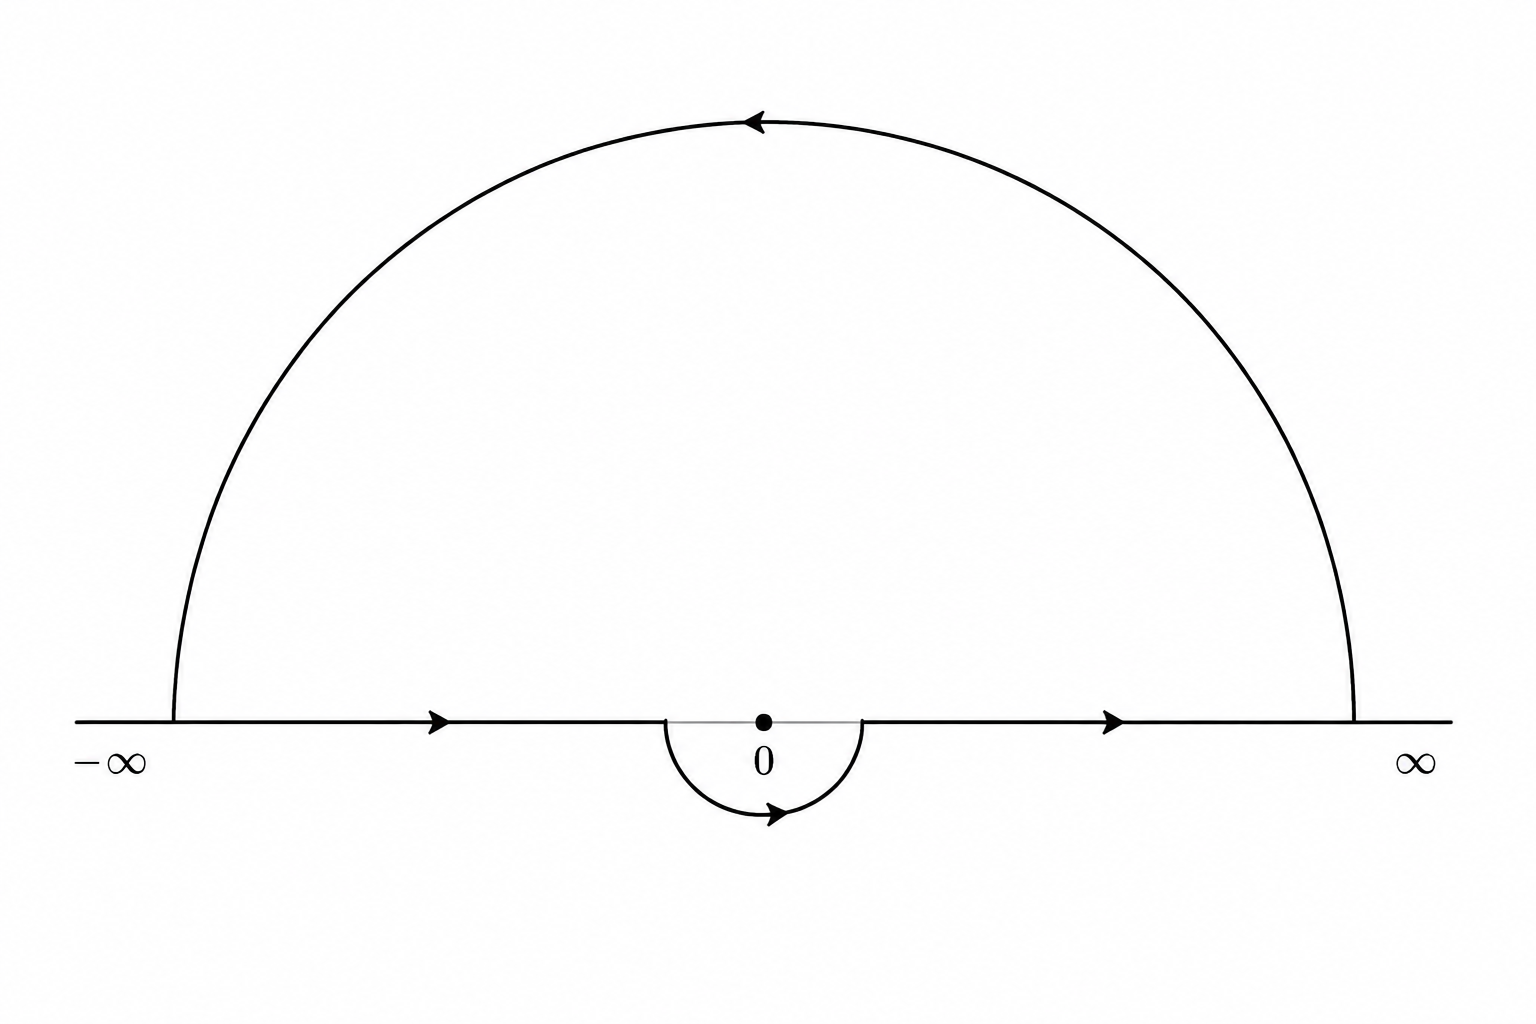
\includegraphics[width = 0.5\textwidth]{integration curve}
		\caption{\textsf{The contour used to evaluate $\mathcal{I}_{3}$ in \eqref{4.110}. We know that the integral along the denoted contour is equal to $2\pi$ times the residues of the integrand in the region bounded by the contour. the singularity of the integrand occurs at $x = 0$ and we need to evaluate the residue at this point.}}
	\end{figure}
	Let us find the residue of the integrand at $x = 0$. In this case, expanding the exponential and then using the Laurent series of the integrand, makes it pretty straightforward to find the resiude. So
	\begin{equation}
		\frac{1}{x^{n+1}}\, e^{ix} = \frac{1}{x^{n+1}}\, \sum_{k = 0}^{\infty} \dfrac{\left( ix \right)^{k}}{k!} = \sum_{k = 0}^{\infty} \dfrac{ i^{k}\, \left( x \right)^{k-n-1}}{k!} \label{4.111}
	\end{equation}
	The residue of the integrand $e^{ix}\, x^{-n-1}$ is simply the coefficient of $x^{-1}$ in its Laurent series expansion; which, in this case, is found by setting $k = n$
	\begin{equation}
		\dfrac{i^{n}}{n!} \notag
	\end{equation}
	Thus, we have
	\begin{equation}
		\mathcal{I}_{3} = \int_{-\infty}^{\infty} dx\, e^{ix}\, x^{-n-1} = 2\pi\, \dfrac{i^{n}}{n!} \label{4.112}
	\end{equation}
	Continuing \eqref{4.110}, we can write
	\begin{equation}
		\tilde{a}_{2}(\infty) = -\sum_{n = 0}^{\infty} \dfrac{n!\, \beta_{n}}{6^{3}\, n^{2}\, i^{n+1}} \times 2\pi\, \dfrac{i^{n}}{n!} = \frac{\pi}{3} \sum_{n = 0}^{\infty} -\frac{\beta_{n}}{36n^{2}} = \frac{\pi}{3} \sum_{n = 0}^{\infty} \alpha_{n} \label{4.113}
	\end{equation}
	By letting $n \rightarrow \infty$ in \eqref{4.105}, we get
	\begin{equation}
		\sum_{n = 0}^{\infty} \alpha_{n} = \lim_{n \rightarrow \infty} -36n^{2} \alpha_{n} = \lim_{n \rightarrow \infty} \beta_{n} = \prod_{m = 1}^{\infty} \left( 1 - \frac{1}{36m^{2}} \right)
	\end{equation}
	Using the Weierstrass product formula for the sine function \cite{Ahlfors1979}, we have
	\begin{equation}
		\sin(\pi z) = \pi z \prod_{m = 1}^{\infty} \left(1 - \frac{z^{2}}{m^{2}} \right) \label{4.115}
	\end{equation}
	Setting $z = \frac{1}{6}$, we get
	\begin{equation}
		\prod_{m = 1}^{\infty} \left( 1 - \frac{1}{36m^{2}} \right) = \frac{6}{\pi} \sin(\frac{\pi}{6}) = \frac{3}{\pi} \label{4.116}
	\end{equation}
	And finally, from \eqref{4.113} we get
	\begin{equation}
		\tilde{a}_{2}(\infty) = \frac{\pi}{3} \times \frac{3}{\pi} = 1 \label{4.117}
	\end{equation}
	Thus, we conclude that $\Gamma_{+} \rightarrow 1$ as $\hbar \rightarrow 0$. Now remember, from \ref{subsec:real analysis} that $a_{1} = \tilde{a}_{1} \rightarrow 1$ as $\hbar \rightarrow 0$. So, using, from \eqref{4.86}, we can write
	\begin{equation}
		\tilde{a}_{1} (\infty) = 1_{-} \tilde{a}_{1}(-\infty) + \Gamma_{-} \tilde{a}_{2}(-\infty) \qquad \rightarrow \qquad 1 = 1_{-} \times 1 + \Gamma_{-} \times 0 \label{4.118}
	\end{equation}
	And thus, we can conclude that $1_{-} \rightarrow 1$ as $\hbar \rightarrow 0$. The diagonal element $1_+$ is obtained from the adiabatic theorem, which guarantees that a system starting in state 2 remains in state 2 in the limit $\hbar \to 0$. Hence, $1_+ \to 1$. To find $\Gamma_{-}$ in the limit where $\hbar \rightarrow 0$, we will carry on as follows: First we define the vectors and the matrices
	\begin{equation}
		\boldsymbol{\tilde{a}}(t) \equiv
		\begin{pmatrix}
			\tilde{a}_{1}(t) \\[5pt]
			\tilde{a}_{2}(t)
		\end{pmatrix} \label{4.119}
	\end{equation}
	And
	\begin{equation}
		\mathbf{A} \equiv
		\begin{pmatrix}
			0 & -\gamma\, e^{-} \\[5pt]
			\gamma\, e^{+} & 0
		\end{pmatrix} \label{4.120}
	\end{equation}
	Writing \eqref{4.18} and \eqref{4.19} in terms of these, will give
	\begin{equation}
		\boldsymbol{\tilde{a}}' = \mathbf{A}\, \boldsymbol{\tilde{a}} \label{4.121}
	\end{equation}
	We define the \emph{fundamental matrix} $\mathbf{T}(t, t_{-})$ as follows:
	\begin{equation}
		\boldsymbol{\tilde{a}}(t) = \mathbf{T}(t, t_{-})\,  \boldsymbol{\tilde{a}}(t_{-}) \label{4.122}
	\end{equation}
	Where
	\begin{equation}
		\mathbf{T}(t_{-}, t_{-}) = \mathbf{I} \label{4.123}
	\end{equation}
	$\mathbf{I}$ is the identity matrix.The fundamental matrix satisfies
	\begin{equation}
		\mathbf{T}'(t, t_{-}) = \mathbf{A}\, \mathbf{T}(t, t_{-}) \label{4.124}
	\end{equation}
	An important relation for the fundamental matrix is given by Liouville's formula (Or Abel-Jacobi-Liouville identity) \cite{CoddingtonLevinson1955}:
	\begin{equation}
		\frac{d}{dt} \mathrm{det} \left[ \mathbf{T}(t, t_{-}) \right] = \mathrm{Tr} \left[ \mathbf{A}(t) \right]\, \mathrm{det} \left[ \mathbf{T}(t, t_{-}) \right] \label{4.125}
	\end{equation}
	Now since the matrix $\mathbf{A}$ given in \eqref{4.120} is traceless, we find that the determinant of the fundamental matrix remains constant in time and follows that
	\begin{equation}
		\mathrm{det} \left[ \mathbf{T}(t, t_{-}) \right] = \mathrm{det} \left[ \mathbf{T}(t_{-}, t_{-}) \right] = \mathrm{det}[ \mathbf{I}] = 1 \label{4.126}
	\end{equation}
	It is evident that, from equation \eqref{4.86}, the limiting transition matrix plays the role of the fundamental matrix in the linear system in \eqref{4.121}. So
	\begin{equation}
		\mathrm{det}
		\begin{pmatrix}
			1_{-} && \Gamma_{-} \\[5pt]
			\Gamma_{+} && 1_{+}	 
		\end{pmatrix} = 1 \Rightarrow 1_{-} 1_{+} - \Gamma_{+} \Gamma_{-} = 1 \label{4.127}
	\end{equation}
	Which gives
	\begin{equation}
		\Gamma_{-} = 0 \label{4.128}
	\end{equation}
	As $\hbar \rightarrow 0$. Having proved the claim in \eqref{4.50}, we will now determine the asymptotic convergence of $a_{2}(\infty)$ and the transition amplitude. From \eqref{4.17} and \eqref{4.117}, we can write
	\begin{equation}
		\boxed{a_{2}(\infty) \sim \exp\left( \frac{i}{\hbar} \Delta_{c} \right)} \label{4.129}
	\end{equation}
	And
	\begin{equation}
		\boxed{\mathcal{P}_{1\rightarrow2} = \left| a_{2}(\infty) \right|^{2} \sim \exp\left( -\frac{2}{\hbar} \mathrm{Im} \left[ \Delta_{c} \right] \right)} \label{4.130}
	\end{equation}
	These remarkable results are what we had set out to prove and, well, here we are!
	
	\section{Discussion} 
	
	We have re-derived the asymptotic form of the nonadiabatic transition amplitude for a two-state quantum system in the semiclassical/adiabatic limit. The main result, given in \eqref{4.129} and \eqref{4.130}, is Dykhne's formula:
	\[
	a_2(+\infty) \sim \exp\left( \frac{i}{\hbar} \Delta_c \right), \qquad 
	\mathcal{P}_{1 \to 2} = |a_2(+\infty)|^2 \sim \exp\left( -\frac{2}{\hbar} \operatorname{Im}[\Delta_c] \right).
	\]
	This result is remarkable for several reasons. First, the transition amplitude depends only on the analytic structure of the energy gap $\delta E(t)$ in the complex time plane — specifically, on the branch point $t_c$ where the two energy levels cross in the complex domain. Second, it is completely independent of the detailed form of the nonadiabatic coupling $\gamma(t)$. The coupling's only role is to determine the location of the branch point; once that is known, the amplitude is universal.
	
	The proof relies on extending the time variable into the complex plane. The avoided crossing on the real axis becomes a true crossing in the complex plane, and the nonadiabatic transition is interpreted as tunneling through the complex-time barrier. The contour deformation method, with the crucial scaling $|t - t_c| = O(\hbar^{2/3 - \epsilon})$, allowed us to localize the transition to the vicinity of $t_c$ and to prove that the remainder terms vanish in the limit $\hbar \to 0$. The universality of the prefactor follows from the universal pole structure of $\gamma(t)$ near $t_c$:
	\[
	\gamma(t) = \frac{1}{4i(t - t_c)} + \eta(t),
	\]
	where the residue $1/(4i)$ is independent of the Hamiltonian.
	
	The result is consistent with the adiabatic theorem for the diagonal elements of the transfer matrix, but it corrects the naive expectation for the off-diagonal element: the transition amplitude is not zero, but exponentially small with a phase. This is the essential content of Dykhne's formula and the central result of the Hwang–Pechukas approach. The method is rigorous and does not rely on perturbation theory beyond the adiabatic basis.
	
	Several extensions and connections should be noted. The complex-time method is not merely a mathematical trick — it provides a physical picture of nonadiabatic transitions as tunneling events in the complex time plane. This perspective has influenced recent work on shortcuts to adiabaticity and counterdiabatic driving, where the adiabatic gauge potential is used to suppress transitions exactly \cite{Cardoso2023}. Generalizations to multi-level systems have been developed by Joye, Kunz, and Pfister \cite{JoyeKunzPfister1991}, who established exponential bounds for the transition probabilities in the general $n$-state case and discussed the geometric nature of the formula. The role of geometric phases in the complex-time method is also an important direction for future work, as the diagonal connection $\langle n|\dot{n}\rangle$ can contribute an additional phase when the eigenstates are complex.
	
	The analysis is restricted to two-state systems and assumes that the Hamiltonian is analytic and that the closest branch point is a simple square-root singularity. The assumption that $\gamma$, $(\gamma/\delta E)'$, and $\gamma^2/\delta E$ are absolutely integrable along the real axis and the level lines is also essential. Despite these limitations, the Hwang–Pechukas method provides a powerful and elegant framework for understanding nonadiabatic transitions. Its connection to the adiabatic gauge potential and to shortcuts to adiabaticity suggests that it remains relevant to modern quantum physics. The Landau-Zener formula, recovered as a special case of Dykhne's formula, remains a cornerstone of quantum control and quantum computing.
	
	In summary, the complex-time approach offers a rigorous and physically transparent derivation of nonadiabatic transition amplitudes. It bridges the adiabatic theorem, complex analysis, and semiclassical physics, and continues to inspire new developments in quantum dynamics.
	
	In summary, we have re-derived Dykhne's formula for the nonadiabatic transition amplitude in a two-state system. The derivation assumes the adiabatic theorem for the diagonal elements of the transfer matrix and computes the off-diagonal element $\Gamma_+$ explicitly via contour integration and steepest descent. The result shows that the transition amplitude depends only on the complex branch point $t_c$ of the energy gap and is independent of the detailed form of the nonadiabatic coupling. This establishes the asymptotic form of the transition probability in the semiclassical/adiabatic limit and confirms the validity of the Hwang–Pechukas approach.

	\newpage
	\phantomsection
	\label{sec:References}
	\addcontentsline{toc}{section}{References}
	\begin{thebibliography}{99}
		
		\bibitem{Zener1932}
		C.~Zener,
		\href{https://doi.org/10.1098/rspa.1932.0165}{\textit{Nonadiabatic crossing of energy levels}},
		Proc. R. Soc. Lond. A \textbf{137}, 696 (1932).
		
		\bibitem{CoddingtonLevinson1955}
		E.~A.~Coddington and N.~Levinson,
		\textit{Theory of Ordinary Differential Equations},
		(McGraw-Hill, New York, 1955).
		
		\bibitem{Dykhne1962}
		A.~M.~Dykhne,
		\href{https://jetp.ras.ru/cgi-bin/dn/e_014_04_0941.pdf}{\textit{Adiabatic perturbation of discrete spectrum states}},
		Sov. Phys. JETP \textbf{14}, 941 (1962).
		
		\bibitem{DavisPechukas1976}
		J.~P. Davis and P.~Pechukas,
		\href{https://doi.org/10.1063/1.432648}{\textit{Nonadiabatic transitions induced by a time-dependent Hamiltonian in the semiclassical/adiabatic limit: The two-state case}},
		J. Chem. Phys. \textbf{64}, 3129 (1976).
		
		\bibitem{Ahlfors1979}
		L.~V.~Ahlfors,
		\textit{Complex Analysis},
		3rd ed. (McGraw-Hill, New York, 1979).
		
		\bibitem{HwangPechukas1977}
		J.~T. Hwang and P.~Pechukas,
		\href{https://doi.org/10.1063/1.434630}{\textit{The adiabatic theorem in the complex plane and the semiclassical calculation of nonadiabatic transition amplitudes}},
		J. Chem. Phys. \textbf{67}, 4640 (1977).
		
		\bibitem{JoyeKunzPfister1991}
		A.~Joye, H.~Kunz, and C.-E.~Pfister,
		\href{https://doi.org/10.1016/0003-4916(91)90297-L}{\textit{Exponential decay and geometric aspect of transition probabilities in the adiabatic limit}},
		Ann. Phys. (N.Y.) \textbf{208}, 299 (1991).
		
		\bibitem{Merzbacher}
		E.~Merzbacher,
		\textit{Quantum Mechanics},
		3rd ed. (Wiley, New York, 1998).
		
		\bibitem{Zwiebach2018}
		B.~Zwiebach,
		\href{https://ocw.mit.edu/courses/8-06-quantum-physics-iii-spring-2018/95ffb7405e75bec4f75564318e173ce0_MIT8_06S18ch6.pdf}{\textit{Adiabatic approximation (Chapter 6)}},
		MIT 8.06 Quantum Physics III Lecture Notes (2018).
		
		\bibitem{Cardoso2023}
		G.~Cardoso,
		\href{https://arxiv.org/abs/2303.12066}{\textit{A Landau-Zener formula for the Adiabatic Gauge Potential}},
		arXiv:2303.12066 (2023).
		
	\end{thebibliography}
	
\end{document}